\documentclass[../Thesis-IJspeert.tex]{subfiles}

\begin{document}

\graphicspath{ {"Cavity Compatible Trapping Architectures/figs/"} }
\pgfplotsset{table/search path={"Cavity Compatible Trapping Architectures/data/"}}

\chapter{Cavity Compatible Trapping Architectures}
\addtocontents{toc}{\vskip-6pt\par\noindent\protect\textcolor{gray75}{\protect\rule{\textwidth}{0.5pt}}\par}
\label{chap:CavityCompatibleTrappingArchitectures}

\section{CAVITY MOUNTING FINGER DESIGN}
In the current setup for cavity-assisted photon generation \cite{Barrett2019}, atoms are loaded stochastically into the cavity mode via an atomic fountain. However, the cavity used in that experiment (with a geometry as shown in \autoref{fig:cavity}) is not compatible with holographic optical tweezers, since its mirrors are relatively large ($\diameter \SI{1.5}{\milli\meter}$) in comparison to the length of the cavity (\SI{339}{\micro\meter}). These dimensions imply that the full accessible angle of this cavity is \ang{25.5}, whereas the trapping light would propagate through the glass cell at nearly the full acceptance angle of the high numerical aperture lens, which is \ang{73.7}. A new cavity is under construction which consists of two truncated square pyramids of silica. An important difference is that the surfaces of truncation are much smaller ($\SI{300}{\micro\meter}\times\SI{300}{\micro\meter}$). This implies that for a similar cavity length ($\sim\SI{300}{\micro\meter}$), the new design would feature a full accessible angle of \ang{90}, which is compatible with the current optical tweezers. Another difference is the method of cavity mirror fabrication. In the current design, the macroscopic silica substrates are super-polished, which means that these mirrors can have exceptionally low losses ($\sim\SI{2}{ppm}$). The disadvantage of this technique is that it results in a relatively large radius of curvature (\SI{50}{\milli\meter}) and mirror diameter. An alternative approach involves the use of intense \ce{CO2} laser pulses to ablate Gaussian micro-dimples onto the end facets of optical fibres \cite{Hunger2010}, which yields a much smaller radius of curvature (\SI{200}{\micro\meter} within a range varying from \SI{50}{\micro\meter} to \SI{1}{\milli\meter}) that can enable a smaller mode volume and therefore higher cooperativity. However, fibre-based optical microcavities can be difficult to stabilise due to the limited mass of the fibre and the fact that the cavity facets are always under some tension from the rest of the structure \cite{Janitz2017}. Another complication is the limited spatial mode matching between the cavity mode and the input/output modes of the fibre. In the new cavity design, the ablation is performed on the truncated surfaces of the macroscopic silica bases for increased stability and improved mode matching, whilst incorporating the advantages of an ablated mirror surface.




\begin{figure}[!t]
	%\vspace{0.7em}
	\centering
	\begin{tikzpicture}
	
	\begin{groupplot}[group style={group size=1 by 3, vertical sep=1cm},xmin=0,ymin=0,height=5.5cm,width=13.5cm,no markers]
	
	\iffalse
	\nextgroupplot
	[
	ylabel={},
	xmin=0, xmax=1,
	ymin=0, ymax=1,
	xticklabels={,\textcolor{white}{0},},
	yticklabels={,,},
	%legend pos=north west,
	ymajorgrids=true,
	xmajorgrids=true,
	grid style=dashed,
	%axis lines=none,        % No axis lines
	%tick style=none,        % No ticks
	%xtick=\empty,           % No x-axis ticks
	%ytick=\empty,           % No y-axis ticks
	xlabel={},              % No x-axis label
	ylabel={},              % No y-axis label
	%enlargelimits=true,     % Keeps the plot within the bounds
	]
	
	\addplot graphics [
	xmin=0, xmax=1,  % Stretch to fit the x-axis limits
	ymin=0, ymax=1    % Stretch to fit the y-axis limits
	] {FINALFINGER.png};
	\fi
	
	
	\nextgroupplot
	[
	ymode=log,
	ymin=1e-0,
	ymax=1e4,
	%xlabel={Frequency},
	%ylabel={Max. linear acceleration},
	xmin=0, xmax=10,
	xticklabels={,,},
	%ymin=-0.1, ymax=1.1,
	%ymin=0, ymax=120,
	%xtick={0,20,40,60,80,100},
	%ytick={0,20,40,60,80,100,120},
	%legend pos=north west,
	ymajorgrids=true,
	xmajorgrids=true,
	grid style=dashed,
	legend cell align={left},
	legend style={
		at={(1, 1)},  % Adjust (x, y) to move it
		anchor=north east,  % Attach the legend to its top-right corner
		draw=none,           % Optional: Remove border around the legend
		fill=none,
		align=left
	}
	]
	
	%\node[align=center] at (axis cs: 0.267, 3500) {\footnotesize A};
	\node[align=center] at (axis cs: 1.105, 3500) {\footnotesize\sc b};
	\node[align=center] at (axis cs: 1.254+0.2, 11) {\footnotesize\sc c};
	\node[align=center] at (axis cs: 2.940, 2000) {\footnotesize\sc d};
	%\node[align=center] at (axis cs: 3.024, 2500) {\footnotesize E};
	\node[align=center] at (axis cs: 3.893, 1500) {\footnotesize\sc f};
	%\node[align=center] at (axis cs: 6.643, 300) {\footnotesize G};
	\node[align=center] at (axis cs: 6.935, 1600) {\footnotesize\sc h};
	
	
	\addplot[
	color=markrood,
	name path=xpointone,
	] table [col sep = comma, x expr = \thisrowno{0}/1000, y index = 1]{M_x_01.csv};
	
	\addplot[
	color=rainbow2of8,
	name path=xone,
	] table [col sep = comma, x expr = \thisrowno{0}/1000, y index = 1]{M_x_1.csv};
	
	\addplot[
	color=rainbow3of8,
	name path=xfive,
	] table [col sep = comma, x expr = \thisrowno{0}/1000, y index = 1]{M_x_5.csv};
	
	\addplot+[draw=none,domain=0:10,name path=xzero] {0.01}; 
	
	\addplot[color=markrood, opacity=0.5] fill between[
	of = xone and xpointone,
	]; 
	
	\addplot[color=rainbow2of8, opacity=0.5] fill between[
	of = xfive and xone,
	]; 
	
	\addplot[color=rainbow3of8, opacity=0.5] fill between[
	of = xzero and xfive,
	]; 
	
	\node at (rel axis cs: 0.52, 0.65) [anchor=center] {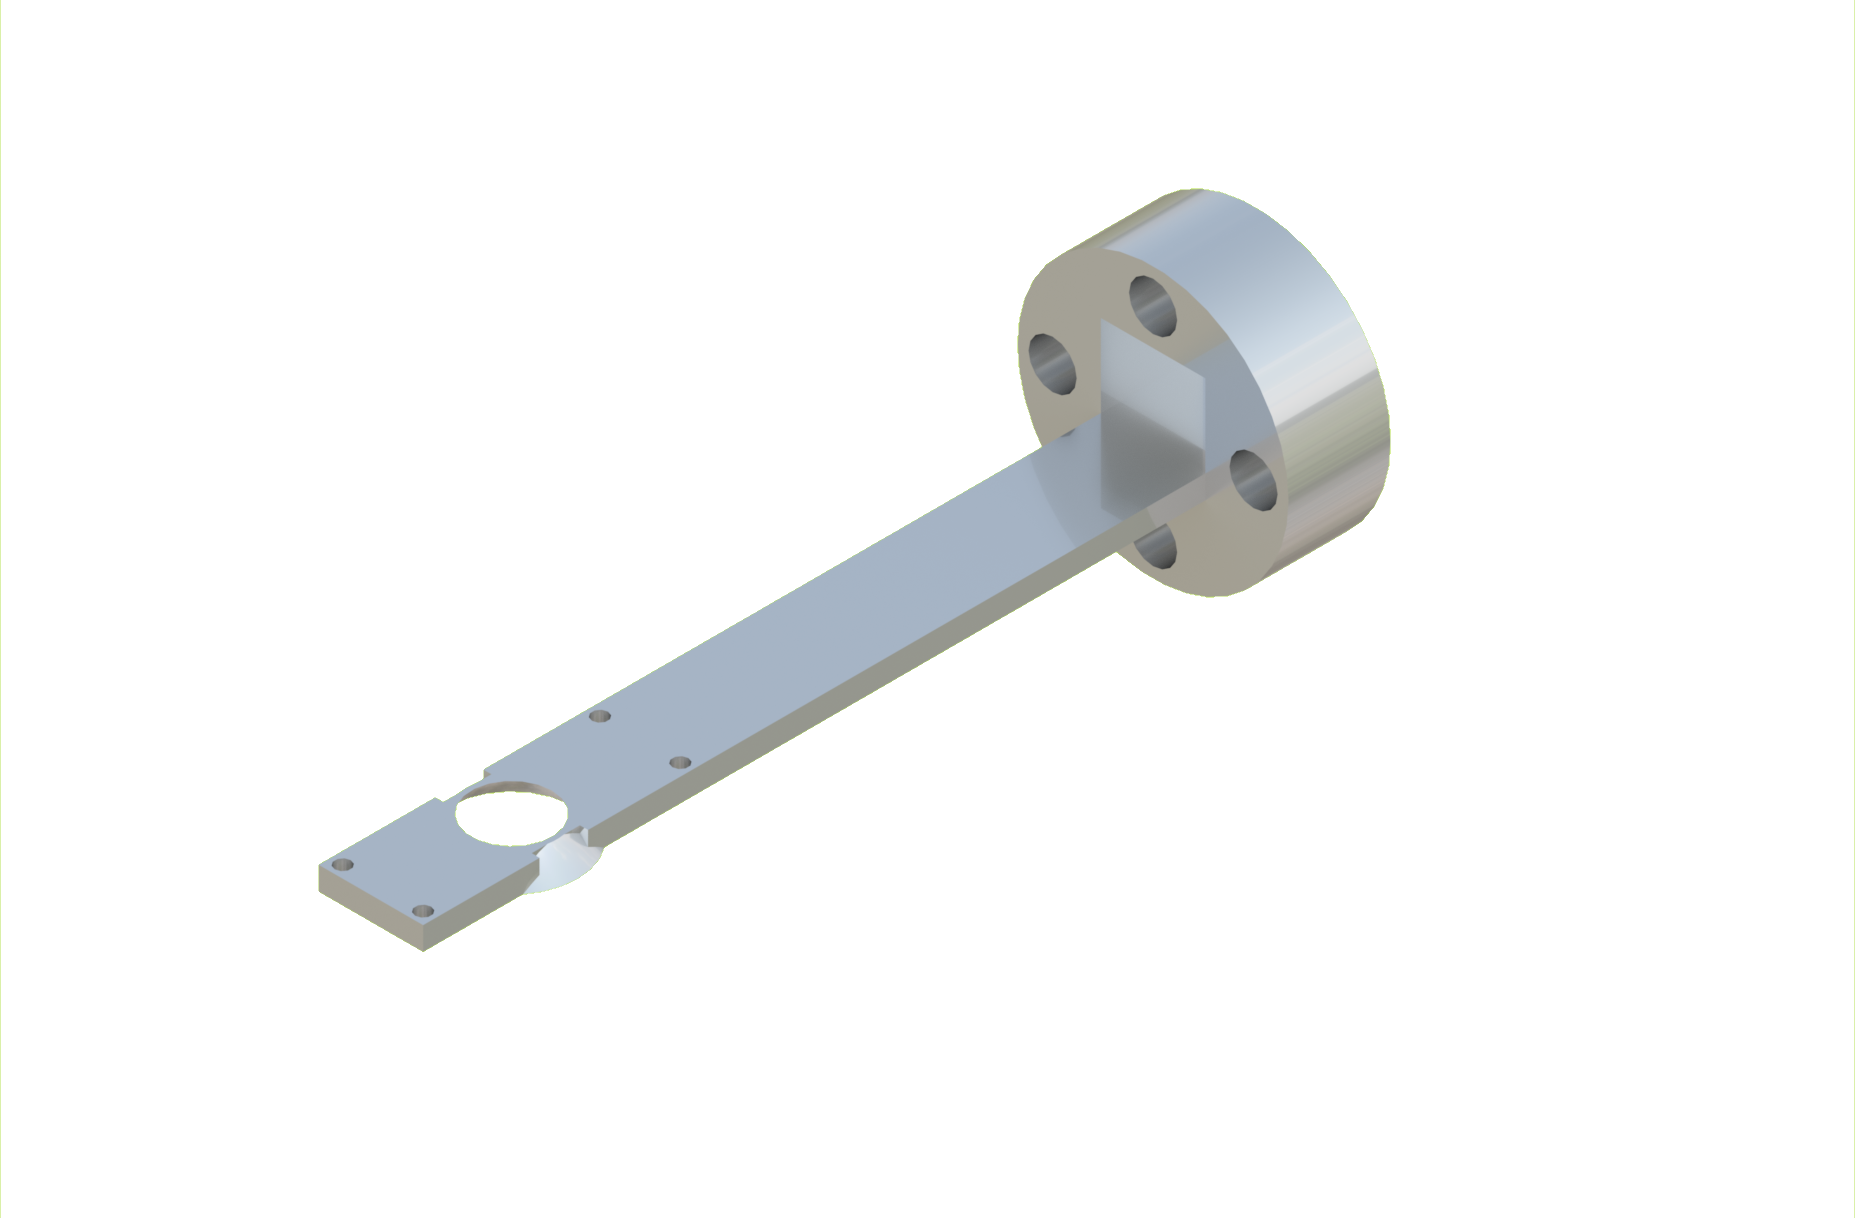
\includegraphics[width=3.5cm]{MARWANFINGERtrans.png}};
	
	\addlegendentry{\footnotesize \hspace{0.3em} $G=\SI{0.1}{\percent}$}
	\addlegendentry{\footnotesize \hspace{0.3em} $G=\SI{1}{\percent}$}
	\addlegendentry{\footnotesize \hspace{0.3em} $G=\SI{5}{\percent}$}
	
	\draw[thick, <->] (rel axis cs: 0.64, 0.8) --++ (150:0.5cm);
	\node[align=left] at (rel axis cs: 0.632, 0.88) {\footnotesize $x$};
	
	\nextgroupplot
	[
	ymode=log,
	ymin=1e-0,
	ymax=1e3,
	%ymin=1e-2, ymax=1e0,
	%xlabel={Frequency},
	ylabel={Maximum linear acceleration magnitude (\si{\milli\meter\per\second\squared})},
	xmin=0, xmax=10,
	xticklabels={,,},
	%ymin=-0.1, ymax=1.1,
	%ymin=0, ymax=120,
	%xtick={0,20,40,60,80,100},
	%ytick={0,20,40,60,80,100,120},
	%legend pos=north west,
	ymajorgrids=true,
	xmajorgrids=true,
	grid style=dashed,
	legend cell align={left},
	legend style={
		at={(1, 1)},  % Adjust (x, y) to move it
		anchor=north east,  % Attach the legend to its top-right corner
		draw=none,           % Optional: Remove border around the legend
		fill=none,
		align=left
	}
	]
	
	\node[align=center] at (axis cs: 0.267, 2.8) {\footnotesize\sc a};
	%\node[align=center] at (axis cs: 1.105, 3500) {\footnotesize B};
	\node[align=center] at (axis cs: 1.254, 33) {\footnotesize\sc c};
	\node[align=center] at (axis cs: 2.940-0.2, 2) {\footnotesize\sc d};
	\node[align=center] at (axis cs: 3.024, 43) {\footnotesize\sc e};
	\node[align=center] at (axis cs: 3.893, 2.5) {\footnotesize\sc f};
	\node[align=center] at (axis cs: 6.643, 320) {\footnotesize\sc g};
	%\node[align=center] at (axis cs: 6.935, 300) {\footnotesize H};
	
	\addplot[
	color=markrood,
	name path=ypointone,
	] table [col sep = comma, x expr = \thisrowno{0}/1000, y index = 1]{M_y_01.csv};
	
	\addplot[
	color=rainbow2of8,
	name path=yone,
	] table [col sep = comma, x expr = \thisrowno{0}/1000, y index = 1]{M_y_1.csv};
	
	\addplot[
	color=rainbow3of8,
	name path=yfive,
	] table [col sep = comma, x expr = \thisrowno{0}/1000, y index = 1]{M_y_5.csv};
	
	\addplot+[draw=none,domain=0:10,name path=yzero] {0.01}; 
	
	\addplot[color=markrood, opacity=0.5] fill between[
	of = yone and ypointone,
	]; 
	
	\addplot[color=rainbow2of8, opacity=0.5] fill between[
	of = yfive and yone,
	]; 
	
	\addplot[color=rainbow3of8, opacity=0.5] fill between[
	of = yzero and yfive,
	]; 
	
	\node at (rel axis cs: 0.52, 0.65) [anchor=center] {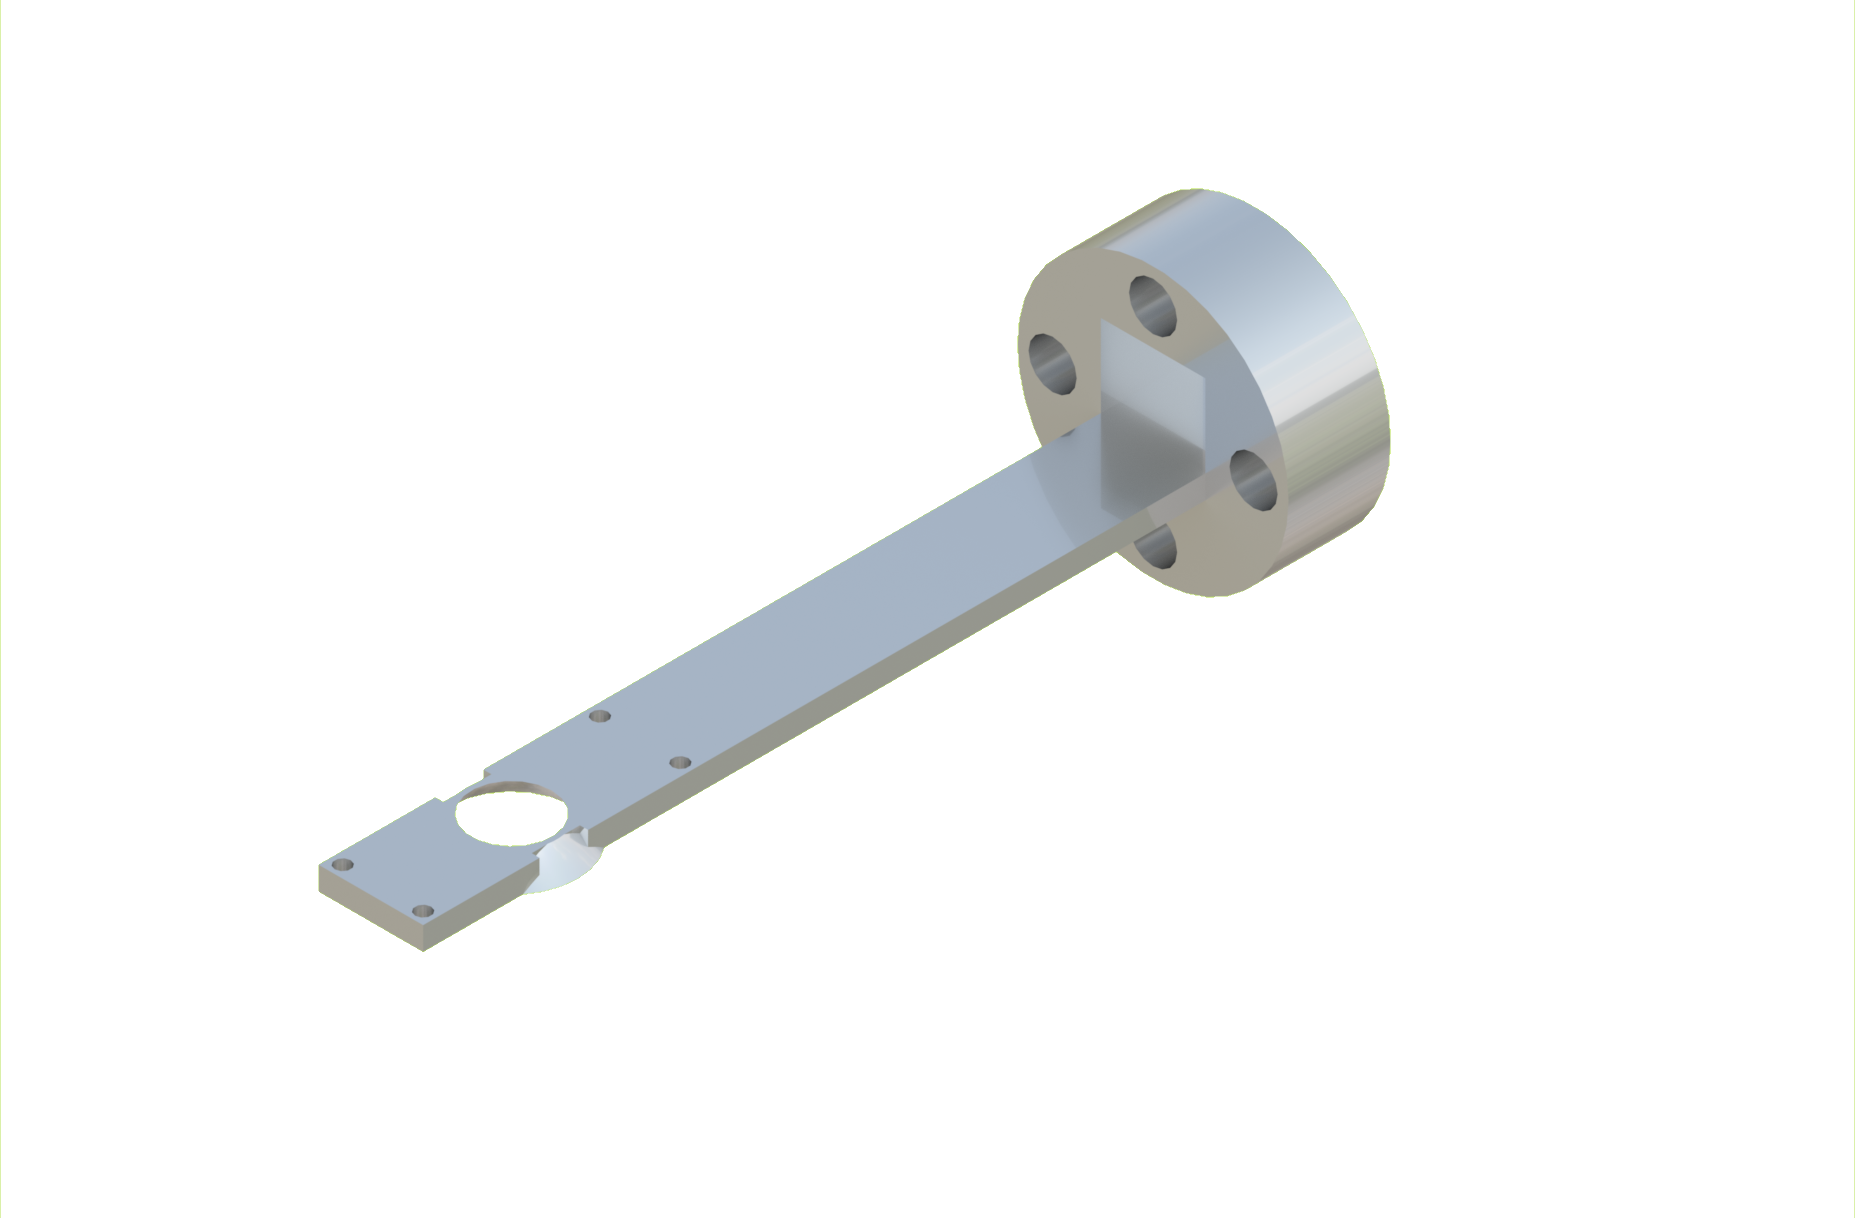
\includegraphics[width=3.5cm]{MARWANFINGERtrans.png}};

	%\addlegendentry{\small \hspace{0.3em} $G=\SI{0.1}{\percent}$}
	%\addlegendentry{\small \hspace{0.3em} $G=\SI{1}{\percent}$}
	%\addlegendentry{\small \hspace{0.3em} $G=\SI{5}{\percent}$}
	
	\draw[thick, <->] (rel axis cs: 0.605, 0.81) --++ (30:0.5cm);
	\node[align=left] at (rel axis cs: 0.615, 0.895) {\footnotesize $y$};
	
	\nextgroupplot
	[
	ymode=log,
	ymin=1e-0,
	ymax=1e4,
	%ymin=1e-2, ymax=1e0,
	xlabel={Enforced acceleration frequency (\si{\kilo\hertz})},
	%ylabel={Max. linear acceleration},
	xmin=0, xmax=10,
	%ymin=-0.1, ymax=1.1,
	%ymin=0, ymax=120,
	%xtick={0,20,40,60,80,100},
	%ytick={0,20,40,60,80,100,120},
	%legend pos=north west,
	ymajorgrids=true,
	xmajorgrids=true,
	grid style=dashed,
	legend cell align={left},
	legend style={
		at={(1, 1)},  % Adjust (x, y) to move it
		anchor=north east,  % Attach the legend to its top-right corner
		draw=none,           % Optional: Remove border around the legend
		fill=none,
		align=left
	}
	]
	
	\node[align=center] at (axis cs: 0.267, 3500) {\footnotesize\sc a};
	%\node[align=center] at (axis cs: 1.105, 3500) {\footnotesize B};
	\node[align=center] at (axis cs: 1.254, 2200) {\footnotesize\sc c};
	\node[align=center] at (axis cs: 2.940-0.2, 30) {\footnotesize\sc d};
	\node[align=center] at (axis cs: 3.024, 1600) {\footnotesize\sc e};
	\node[align=center] at (axis cs: 3.893, 4.5) {\footnotesize\sc f};
	\node[align=center] at (axis cs: 6.643, 1500) {\footnotesize\sc g};
	%\node[align=center] at (axis cs: 6.935, 300) {\footnotesize H};
	
	\addplot[
	color=markrood,
	name path=zpointone,
	] table [col sep = comma, x expr = \thisrowno{0}/1000, y index = 1]{M_z_01.csv};
	
	\addplot[
	color=rainbow2of8,
	name path=zone,
	] table [col sep = comma, x expr = \thisrowno{0}/1000, y index = 1]{M_z_1.csv};
	
	\addplot[
	color=rainbow3of8,
	name path=zfive,
	] table [col sep = comma, x expr = \thisrowno{0}/1000, y index = 1]{M_z_5.csv};
	
	\addplot+[draw=none,domain=0:10,name path=zzero] {0.01}; 
	
	\addplot[color=markrood, opacity=0.5] fill between[
	of = zone and zpointone,
	]; 
	
	\addplot[color=rainbow2of8, opacity=0.5] fill between[
	of = zfive and zone,
	]; 
	
	\addplot[color=rainbow3of8, opacity=0.5] fill between[
	of = zzero and zfive,
	]; 
	
	\node at (rel axis cs: 0.52, 0.65) [anchor=center] {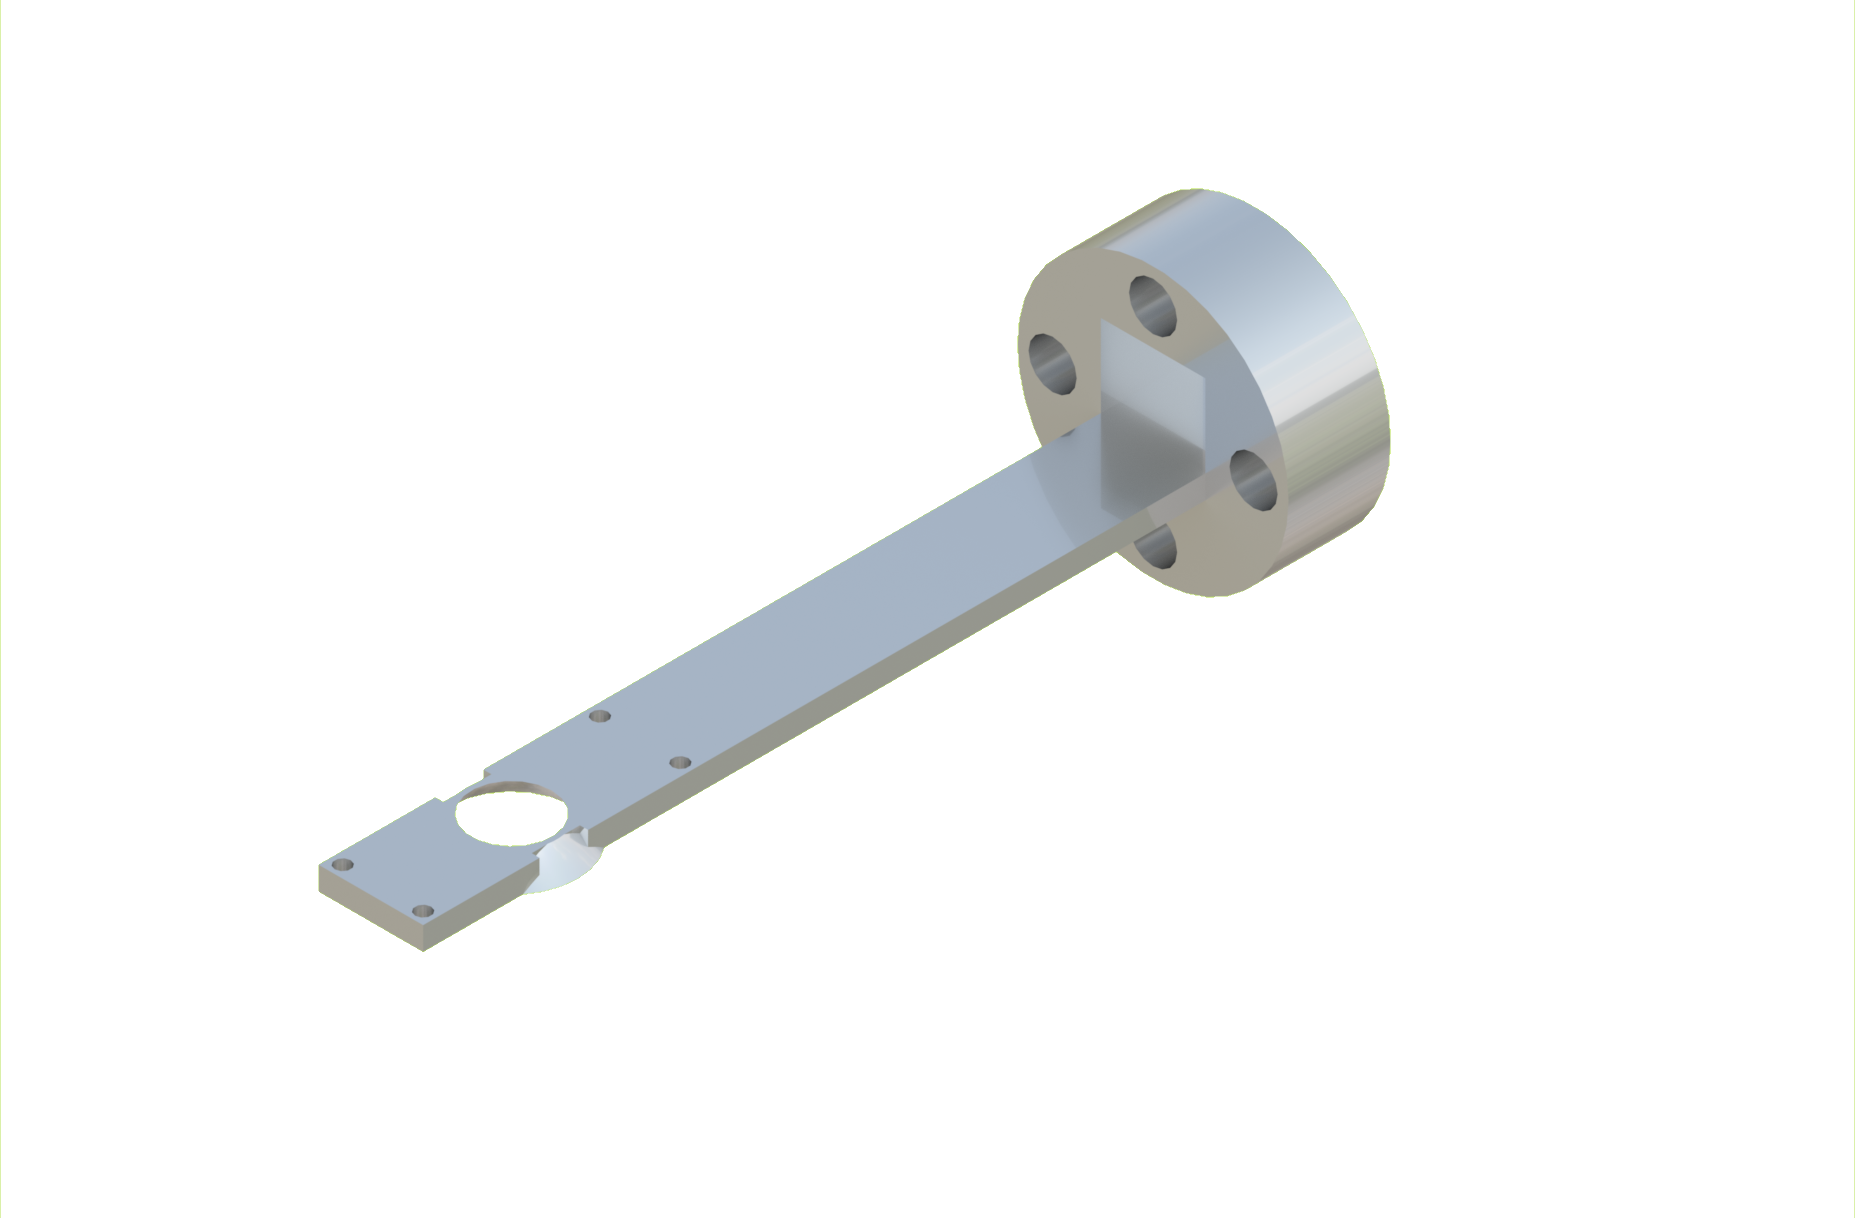
\includegraphics[width=3.5cm]{MARWANFINGERtrans.png}};

	\draw[thick, <->] (rel axis cs: 0.615, 0.79) --++ (90:0.5cm);
	\node[align=left] at (rel axis cs: 0.635, 0.86) {\footnotesize $z$};
	
	
	\end{groupplot}
	
	
	
	\end{tikzpicture}
	\caption[Modal frequency response analysis for fibre-tip cavity mounting structure]{Modal frequency response analysis for fibre-tip cavity mounting structure. The graphs show the maximum linear acceleration magnitude of the structure versus the frequency of enforced acceleration at the base in three different directions: $x$ (top), $y$ (middle) and $z$ (bottom). In each direction, traces are shown for three different values of the structural damping coefficient $G$. The magnitude of the enforced acceleration equals \SI{1}{\milli\meter\per\second\squared}}
	\label{freqresponseMarw} 
\end{figure}



\begin{figure}[t]
	\vspace{0em}
	\centering
	\begin{subfigure}[b]{.45\linewidth}
		\begin{tikzpicture}
		\centering
		\node[inner sep=0] (image) at (0,0) {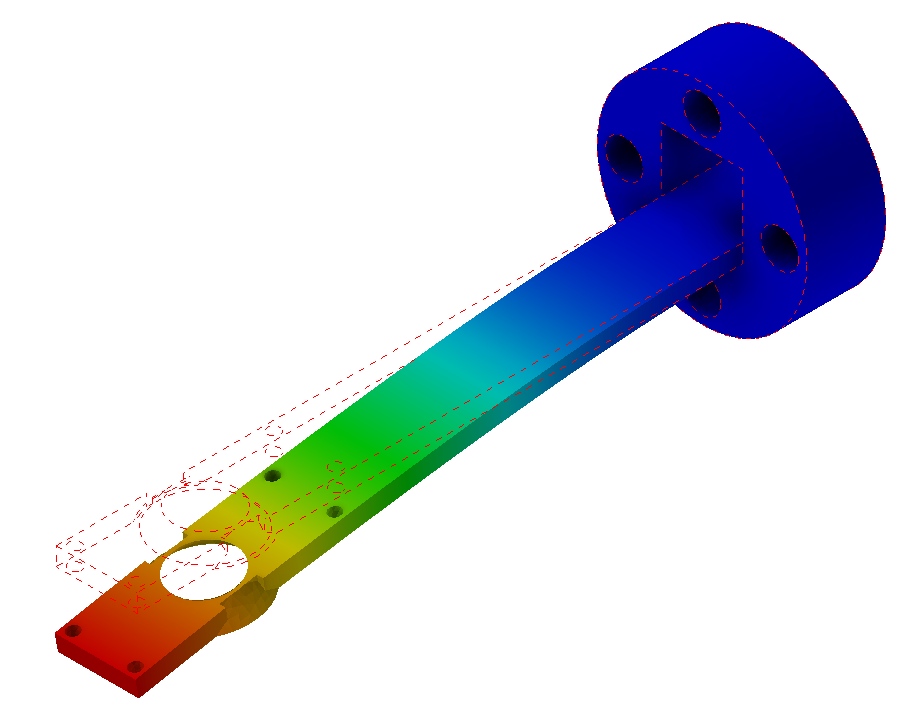
\includegraphics[width=5cm] {1F.png}};;
		\begin{scope}[x={(image.south east)},y={(image.north west)}]
		\node at (0.3, 0.7) {\footnotesize \SI{267}{\hertz}};
		\end{scope}
		\end{tikzpicture}
		\centering
		\caption{}
		\label{a}
	\end{subfigure}
	\begin{subfigure}[b]{.45\linewidth}
		\begin{tikzpicture}
		\centering
		\node[inner sep=0] (image) at (0,0) {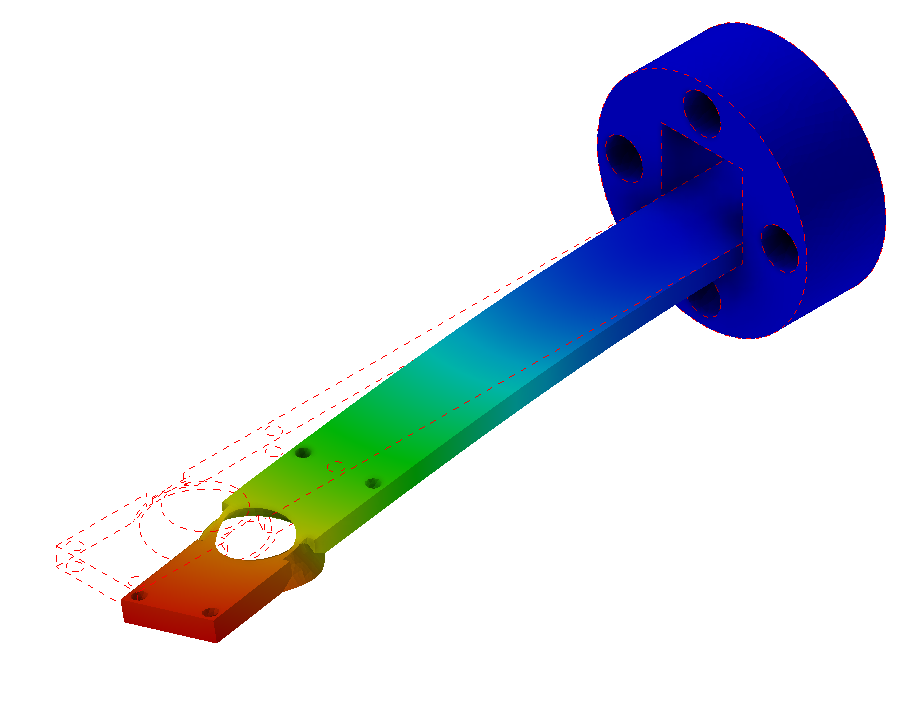
\includegraphics[width=5cm] {2F.png}};;
		\begin{scope}[x={(image.south east)},y={(image.north west)}]
		\node at (0.3, 0.7) {\footnotesize \SI{1105}{\hertz}};
		\end{scope}
		\end{tikzpicture}
		\centering
		\caption{}
		\label{b}
	\end{subfigure}
	\\
	\begin{subfigure}[b]{.45\linewidth}
		\begin{tikzpicture}
		\centering
		\node[inner sep=0] (image) at (0,0) {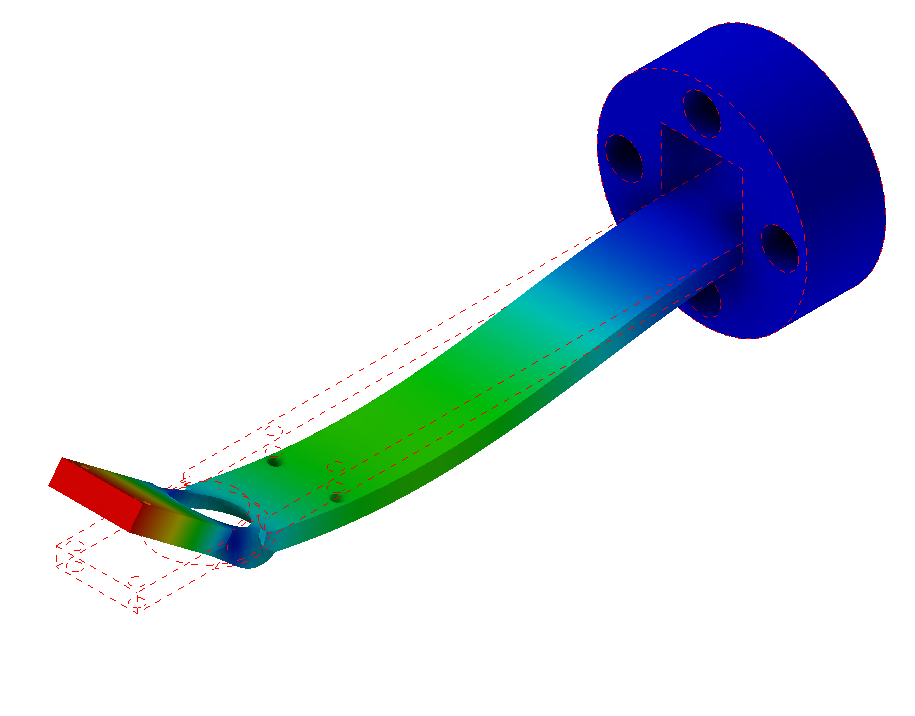
\includegraphics[width=5cm] {3F.png}};;
		\begin{scope}[x={(image.south east)},y={(image.north west)}]
		\node at (0.3, 0.7) {\footnotesize \SI{1254}{\hertz}};
		\end{scope}
		\end{tikzpicture}
		\centering
		\caption{}
		\label{c}
	\end{subfigure}
	\begin{subfigure}[b]{.45\linewidth}
		\begin{tikzpicture}
		\centering
		\node[inner sep=0] (image) at (0,0) {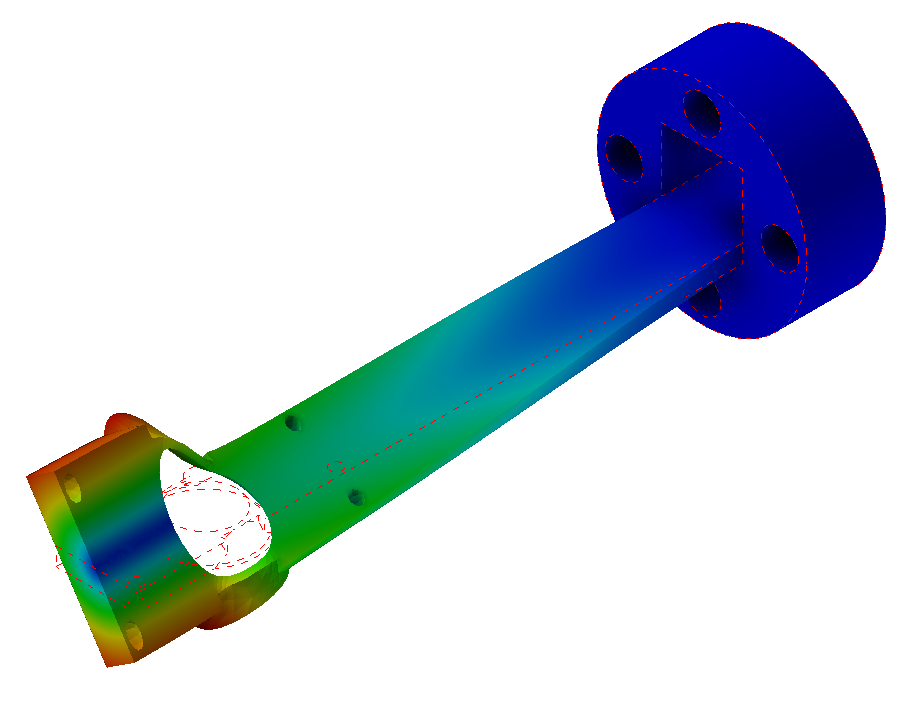
\includegraphics[width=5cm] {4F.png}};;
		\begin{scope}[x={(image.south east)},y={(image.north west)}]
		\node at (0.3, 0.7) {\footnotesize \SI{2940}{\hertz}};
		\end{scope}
		\end{tikzpicture}
		\centering
		\caption{}
		\label{c}
	\end{subfigure}
	\\
	\begin{subfigure}[b]{.45\linewidth}
		\begin{tikzpicture}
		\centering
		\node[inner sep=0] (image) at (0,0) {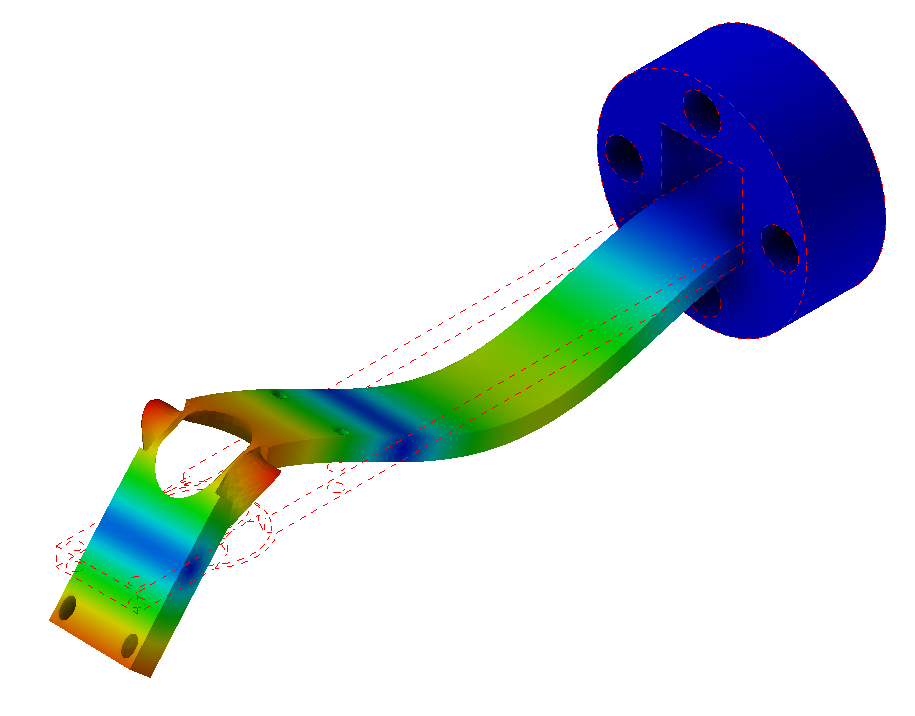
\includegraphics[width=5cm] {5F.png}};;
		\begin{scope}[x={(image.south east)},y={(image.north west)}]
		\node at (0.3, 0.7) {\footnotesize \SI{3024}{\hertz}};
		\end{scope}
		\end{tikzpicture}
		\centering
		\caption{}
		\label{a}
	\end{subfigure}
	\begin{subfigure}[b]{.45\linewidth}
		\begin{tikzpicture}
		\centering
		\node[inner sep=0] (image) at (0,0) {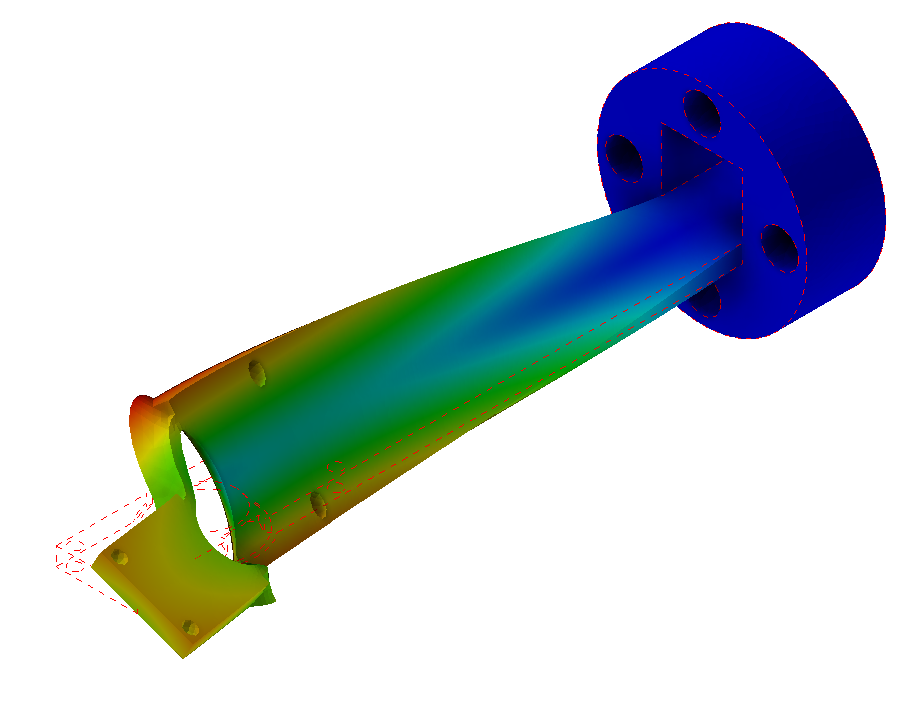
\includegraphics[width=5cm] {6F.png}};;
		\begin{scope}[x={(image.south east)},y={(image.north west)}]
		\node at (0.3, 0.7) {\footnotesize \SI{3893}{\hertz}};
		\end{scope}
		\end{tikzpicture}
		\centering
		\caption{}
		\label{b}
	\end{subfigure}
\\
\begin{subfigure}[b]{.45\linewidth}
	\begin{tikzpicture}
	\centering
	\node[inner sep=0] (image) at (0,0) {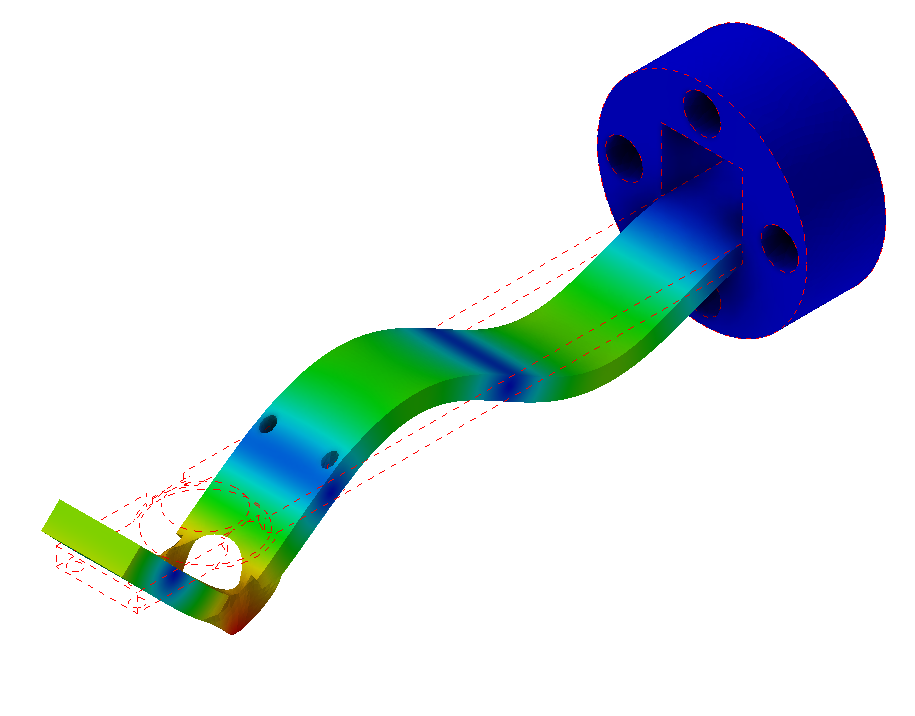
\includegraphics[width=5cm] {7F.png}};;
	\begin{scope}[x={(image.south east)},y={(image.north west)}]
	\node at (0.3, 0.7) {\footnotesize \SI{6643}{\hertz}};
	\end{scope}
	\end{tikzpicture}
	\centering
	\caption{}
	\label{a}
\end{subfigure}
\begin{subfigure}[b]{.45\linewidth}
	\begin{tikzpicture}
	\centering
	\node[inner sep=0] (image) at (0,0) {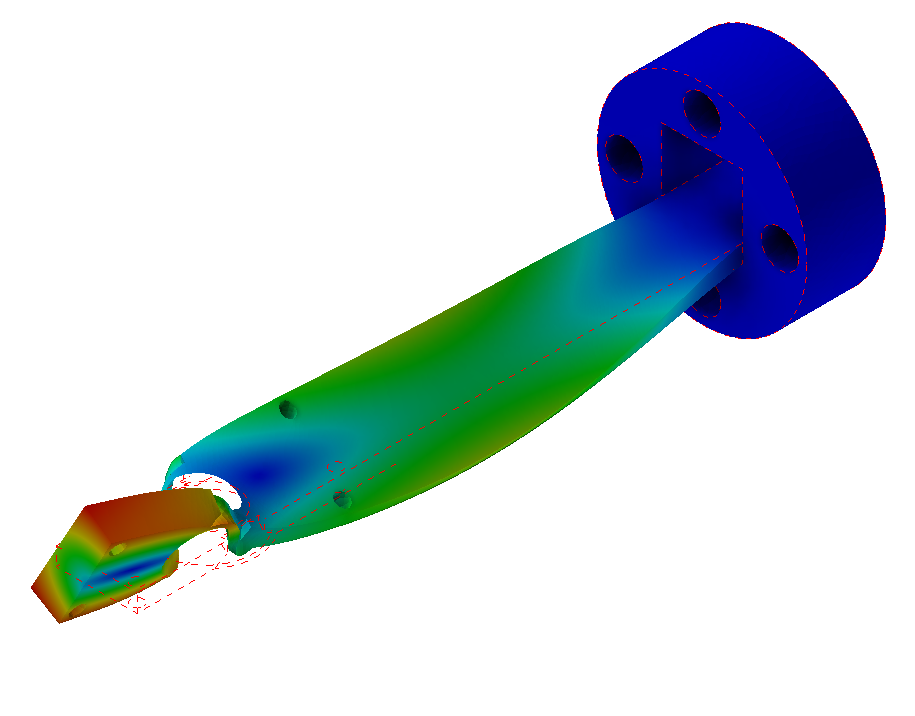
\includegraphics[width=5cm] {8F.png}};;
	\begin{scope}[x={(image.south east)},y={(image.north west)}]
	\node at (0.3, 0.7) {\footnotesize \SI{6935}{\hertz}};
		\draw[thick, ->] (1, 0.15) --++ (90:0.5cm) node[above, anchor=south] {\footnotesize $z$};
\draw[thick, ->] (1, 0.15) --++ (150:0.5cm) node[above, anchor=base] {\footnotesize  $x$\,\, \phantom{x}};
\draw[thick, ->] (1, 0.15) --++ (210:0.5cm) node[above, anchor=mid] {\footnotesize $y$\,\, \phantom{x}};
	\end{scope}
	\end{tikzpicture}
	\centering
	\caption{}
	\label{b}
\end{subfigure}
	\caption[Normal modes below \SI{10}{\kilo\hertz} for fibre-tip cavity mounting structure]{Normal modes and corresponding frequencies below \SI{10}{\kilo\hertz} for the fibre-tip cavity mounting structure. The colour scale corresponds to the displacement from the unperturbed position of the structure (dashed contours). Mode labels correspond to those in \autoref{freqresponseMarw}.}
	\label{marwanmodes}
\end{figure}

\begin{table}[h]
	\centering
	\begin{tabular}{ccccccc}
		\toprule
		{Mode number} & { ${T}_x$} & {${T}_y$} & {${T}_z$} & {${R}_x$} & {${R}_y$} & {${R}_z$} \\
		\midrule
		1 (\textsc{a}) & 0.0000 & 0.0000 & 16.5379 & 85.1071 & 0.0000 & 0.0000 \\
		2 (\textsc{b}) & 15.8373 & 0.0000 & 0.0000 & 0.0000 & 1.8747 & 83.4516 \\
		3 (\textsc{c}) & 0.0001 & 0.0014 & 4.9304 & 4.4790 & 0.0003 & 0.0000 \\
		4 (\textsc{d}) & 1.6181 & 0.0004 & 0.0004 & 0.0002 & 0.5771 & 2.7442 \\
		5 (\textsc{e}) & 0.0001 & 0.0024 & 2.7994 & 1.4686 & 2.7770 & 8.9820 \\
		6 (\textsc{f}) & 2.5962 & 0.0000 & 0.0000 & 0.0322 & 1.1527 & 2.7770 \\
		7 (\textsc{g}) & 0.0000 & 0.1034 & 1.5245 & 0.4678 & 0.0199 & 0.0000 \\
		8 (\textsc{h}) & 1.7830 & 0.0000 & 0.0000 & 0.2995 & 0.0134 & 1.1527 \\
		9 & 3.0222 & 0.0037 & 0.5778 & 0.0001 & 0.7470 & 1.3507 \\
		10 & 0.0005 & 8.4142 & 0.4302 & 0.4197 & 0.0001 & 0.0002 \\
		\midrule
		{Total} & 24.8574 & 8.5251 & 26.2227 & 91.9425 & 5.9831 & 91.5980 \\
		\bottomrule
	\end{tabular}
\caption[Percentages of modal effective mass for cavity (fibre-tip) mounting structure]{Modal effective mass participation for the first 10 modes of the cavity (fibre-tip) mounting structure. The numbers shown represent percentages for the translational (${T}_x$, ${T}_y$, ${T}_z$) and rotational (${R}_x$, ${R}_y$, ${R}_z$) degrees of freedom. Labels are references to the modes as indicated in \autoref{freqresponseMarw} and \autoref{marwanmodes}.}
	\label{modeparticipationM}
\end{table}

\begin{figure}[!t]
	%\vspace{0.7em}
	\centering
	\begin{tikzpicture}
	

	
	\begin{groupplot}[group style={group size=1 by 1, vertical sep=1cm, y descriptions at=edge right,},xmin=0,ymin=0,height=5.5cm,width=12cm,no markers,]
	
	\nextgroupplot
	[
	ymode=log,
	ymin=7e-1,
	ymax=1e4,
	ylabel style=markgrijs,
	yticklabel style=markgrijs,
	%ymin=1e-2, ymax=1e0,
	xlabel={Frequency (\si{\kilo\hertz})},
	ylabel={Max. accel. (\si{\milli\meter\per\second\squared})},
	xmin=0, xmax=10,
	ytick pos=right,
	%ymin=-0.1, ymax=1.1,
	%ymin=0, ymax=120,
	%xtick={0,20,40,60,80,100},
	%ytick={0,20,40,60,80,100,120},
	%legend pos=north west,
	ymajorgrids=true,
	xmajorgrids=false,
	grid style=dashed,
	legend cell align={left},
	legend style={
		at={(1, 1)},  % Adjust (x, y) to move it
		anchor=north east,  % Attach the legend to its top-right corner
		draw=none,           % Optional: Remove border around the legend
		fill=none,
		align=left
	}
	]
	
	\draw[color=markgrijs, dashed] 
	(axis cs:0.267, 7e-1) -- (axis cs:0.267, 40000);
	\draw[color=markgrijs, dashed] 
	(axis cs:1.105, 7e-1) -- (axis cs:1.105, 40000);
	\draw[color=markgrijs, dashed] 
	(axis cs:1.254, 7e-1) -- (axis cs:1.254, 40000);
	\draw[color=markgrijs, dashed] 
	(axis cs:2.940, 7e-1) -- (axis cs:2.940, 40000);
	\draw[color=markgrijs, dashed] 
	(axis cs:3.024, 7e-1) -- (axis cs:3.024, 40000);
	\draw[color=markgrijs, dashed] 
	(axis cs:3.893, 7e-1) -- (axis cs:3.893, 40000);
	\draw[color=markgrijs, dashed] 
	(axis cs:6.643, 7e-1) -- (axis cs:6.643, 40000);
	\draw[color=markgrijs, dashed] 
	(axis cs:6.935, 7e-1) -- (axis cs:6.935, 40000);
	
	
	
	\pgfplotsset{
		after end axis/.append code={
			\node[align=center] at (axis cs: 0.267, 20000) {\footnotesize\sc a};
			\node[align=center] at (axis cs: 1.105-0.06, 20000) {\footnotesize\sc b};
			\node[align=center] at (axis cs: 1.254+0.06, 20000) {\footnotesize\sc c};
			\node[align=center] at (axis cs: 2.940-0.1, 20000) {\footnotesize\sc d};
			\node[align=center] at (axis cs: 3.024+0.1, 20000) {\footnotesize\sc e};
			\node[align=center] at (axis cs: 3.893, 20000) {\footnotesize\sc f};
			\node[align=center] at (axis cs: 6.643, 20000) {\footnotesize\sc g};
			\node[align=center] at (axis cs: 6.935, 20000) {\footnotesize\sc h};
		}
	}
	
	
	
	\addplot[
	color=markgrijs,
	name path=xpointone,
	] table [col sep = comma, x expr = \thisrowno{0}/1000, y index = 1]{M_x_01.csv};
	
	\addplot+[draw=none,domain=0:10,name path=xzero] {1e-11}; 
	
	\addplot[color=markgrijs, opacity=0.1] fill between[
	of = xzero and xpointone,
	]; 
	
	\addplot[
	color=markgrijs,
	name path=ypointone,
	] table [col sep = comma, x expr = \thisrowno{0}/1000, y index = 1]{M_y_01.csv};
	
	\addplot+[draw=none,domain=0:10,name path=yzero] {1e-11}; 
	
	\addplot[color=markgrijs, opacity=0.1] fill between[
	of = yzero and ypointone,
	]; 
	
	\addplot[
	color=markgrijs,
	name path=zpointone,
	] table [col sep = comma, x expr = \thisrowno{0}/1000, y index = 1]{M_z_01.csv};
	
	\addplot+[draw=none,domain=0:10,name path=zzero] {1e-11}; 
	
	\addplot[color=markgrijs, opacity=0.1] fill between[
	of = zzero and zpointone,
	]; 
	
	\end{groupplot}
	
	\begin{groupplot}[group style={group size=1 by 1, vertical sep=1cm,y descriptions at=edge left},xmin=0,ymin=0,height=5.5cm,width=12cm,no markers]
	
	\nextgroupplot
	[
	ymode=log,
	ymin=1e-10,
	ymax=1e-4,
	ylabel style=markrood,
	yticklabel style=markrood,
	every y tick/.style={markrood},
	%ymin=1e-2, ymax=1e0,
	%xlabel={Frequency (\si{\kilo\hertz})},
	ylabel={Power spectral density (\si{\volt\squared\per\hertz})},
	xmin=0, xmax=10,
	%ymin=-0.1, ymax=1.1,
	%ymin=0, ymax=120,
	%xtick={0,20,40,60,80,100},
	%ytick={0,20,40,60,80,100,120},
	%legend pos=north west,
	xtick=\empty,
	axis line style=transparent,
	ytick pos=left,
	ymajorgrids=false,
	xmajorgrids=false,
	grid style=dashed,
	y grid style={color=markrood, opacity=0.3},
	legend cell align={left},
	legend style={
		at={(1, 1)},  % Adjust (x, y) to move it
		anchor=north east,  % Attach the legend to its top-right corner
		draw=none,           % Optional: Remove border around the legend
		fill=none,
		align=left
	}
	]
	
	
	\addplot[
	color=markrood,
	] table [col sep = comma, x expr = \thisrowno{0}/1000, y index = 1]{PSD.csv};
	
	
	\end{groupplot}
	
	\end{tikzpicture}
	\caption[Power spectral density of the fibre-tip cavity transmission signal at \SI{1064}{\nano\meter}]{Power spectral density of the fibre-tip cavity transmission signal at \SI{1064}{\nano\meter}. The grey reference traces correspond to the simulated modal frequency response curves ($x$, $y$ and $z$) as shown in \autoref{freqresponseMarw}. Labels are references to the modes as indicated in \autoref{freqresponseMarw} and \autoref{marwanmodes}.} % The text in the square bracket is the caption for the list of figures while the text in the curly brackets is the figure caption
	\label{PSD} 
\end{figure}

\begin{figure}[!t]
	%\vspace{0.7em}
	\centering
	\begin{tikzpicture}
	
	
	
	\begin{groupplot}[group style={group size=1 by 2, vertical sep=1cm, y descriptions at=edge right,},xmin=0,ymin=0,height=5.5cm,width=12cm,no markers,]
	
	\nextgroupplot
	[
	ymode=log,
	ymin=7e-1,
	ymax=1e4,
	ylabel style=markgrijs,
	yticklabel style=markgrijs,
	%ymin=1e-2, ymax=1e0,
	%xlabel={Frequency (\si{\kilo\hertz})},
	ylabel={Max. accel. (\si{\milli\meter\per\second\squared})},
	xmin=0, xmax=10,
	ytick pos=right,
	xticklabels={,,},
	%ymin=-0.1, ymax=1.1,
	%ymin=0, ymax=120,
	%xtick={0,20,40,60,80,100},
	%ytick={0,20,40,60,80,100,120},
	%legend pos=north west,
	ymajorgrids=true,
	xmajorgrids=false,
	grid style=dashed,
	legend cell align={left},
	legend style={
		at={(1, 1)},  % Adjust (x, y) to move it
		anchor=north east,  % Attach the legend to its top-right corner
		draw=none,           % Optional: Remove border around the legend
		fill=none,
		align=left
	}
	]
	
	\draw[color=markgrijs, dashed] 
	(axis cs:0.267, 7e-1) -- (axis cs:0.267, 40000);
	\draw[color=markgrijs, dashed] 
	(axis cs:1.105, 7e-1) -- (axis cs:1.105, 40000);
	\draw[color=markgrijs, dashed] 
	(axis cs:1.254, 7e-1) -- (axis cs:1.254, 40000);
	\draw[color=markgrijs, dashed] 
	(axis cs:2.940, 7e-1) -- (axis cs:2.940, 40000);
	\draw[color=markgrijs, dashed] 
	(axis cs:3.024, 7e-1) -- (axis cs:3.024, 40000);
	\draw[color=markgrijs, dashed] 
	(axis cs:3.893, 7e-1) -- (axis cs:3.893, 40000);
	\draw[color=markgrijs, dashed] 
	(axis cs:6.643, 7e-1) -- (axis cs:6.643, 40000);
	\draw[color=markgrijs, dashed] 
	(axis cs:6.935, 7e-1) -- (axis cs:6.935, 40000);
	
	
	
	\pgfplotsset{
		after end axis/.append code={
			\node[align=center] at (axis cs: 0.267, 20000) {\footnotesize\sc a};
			\node[align=center] at (axis cs: 1.105-0.06, 20000) {\footnotesize\sc b};
			\node[align=center] at (axis cs: 1.254+0.06, 20000) {\footnotesize\sc c};
			\node[align=center] at (axis cs: 2.940-0.1, 20000) {\footnotesize\sc d};
			\node[align=center] at (axis cs: 3.024+0.1, 20000) {\footnotesize\sc e};
			\node[align=center] at (axis cs: 3.893, 20000) {\footnotesize\sc f};
			\node[align=center] at (axis cs: 6.643, 20000) {\footnotesize\sc g};
			\node[align=center] at (axis cs: 6.935, 20000) {\footnotesize\sc h};
		}
	}
	
	
	
	\addplot[
	color=markgrijs,
	name path=xpointone,
	] table [col sep = comma, x expr = \thisrowno{0}/1000, y index = 1]{M_x_01.csv};
	
	\addplot+[draw=none,domain=0:10,name path=xzero] {1e-11}; 
	
	\addplot[color=markgrijs, opacity=0.1] fill between[
	of = xzero and xpointone,
	]; 
	
	\addplot[
	color=markgrijs,
	name path=ypointone,
	] table [col sep = comma, x expr = \thisrowno{0}/1000, y index = 1]{M_y_01.csv};
	
	\addplot+[draw=none,domain=0:10,name path=yzero] {1e-11}; 
	
	\addplot[color=markgrijs, opacity=0.1] fill between[
	of = yzero and ypointone,
	]; 
	
	\addplot[
	color=markgrijs,
	name path=zpointone,
	] table [col sep = comma, x expr = \thisrowno{0}/1000, y index = 1]{M_z_01.csv};
	
	\addplot+[draw=none,domain=0:10,name path=zzero] {1e-11}; 
	
	\addplot[color=markgrijs, opacity=0.1] fill between[
	of = zzero and zpointone,
	]; 
	
	\nextgroupplot
	[
	ymode=log,
	ymin=7e-1,
	ymax=1e4,
	ylabel style=markgrijs,
	yticklabel style=markgrijs,
	%ymin=1e-2, ymax=1e0,
	xlabel={Frequency (\si{\kilo\hertz})},
	ylabel={Max. accel. (\si{\milli\meter\per\second\squared})},
	xmin=0, xmax=10,
	ytick pos=right,
	%ymin=-0.1, ymax=1.1,
	%ymin=0, ymax=120,
	%xtick={0,20,40,60,80,100},
	%ytick={0,20,40,60,80,100,120},
	%legend pos=north west,
	ymajorgrids=true,
	xmajorgrids=false,
	grid style=dashed,
	legend cell align={left},
	legend style={
		at={(1, 1)},  % Adjust (x, y) to move it
		anchor=north east,  % Attach the legend to its top-right corner
		draw=none,           % Optional: Remove border around the legend
		fill=none,
		align=left
	}
	]
	
	\draw[color=markgrijs, dashed] 
	(axis cs:0.267, 7e-1) -- (axis cs:0.267, 40000);
	\draw[color=markgrijs, dashed] 
	(axis cs:1.105, 7e-1) -- (axis cs:1.105, 40000);
	\draw[color=markgrijs, dashed] 
	(axis cs:1.254, 7e-1) -- (axis cs:1.254, 40000);
	\draw[color=markgrijs, dashed] 
	(axis cs:2.940, 7e-1) -- (axis cs:2.940, 40000);
	\draw[color=markgrijs, dashed] 
	(axis cs:3.024, 7e-1) -- (axis cs:3.024, 40000);
	\draw[color=markgrijs, dashed] 
	(axis cs:3.893, 7e-1) -- (axis cs:3.893, 40000);
	\draw[color=markgrijs, dashed] 
	(axis cs:6.643, 7e-1) -- (axis cs:6.643, 40000);
	\draw[color=markgrijs, dashed] 
	(axis cs:6.935, 7e-1) -- (axis cs:6.935, 40000);
	
	
	
	\pgfplotsset{
		after end axis/.append code={
			\node[align=center] at (axis cs: 0.267, 20000) {\footnotesize\sc a};
			\node[align=center] at (axis cs: 1.105-0.06, 20000) {\footnotesize\sc b};
			\node[align=center] at (axis cs: 1.254+0.06, 20000) {\footnotesize\sc c};
			\node[align=center] at (axis cs: 2.940-0.1, 20000) {\footnotesize\sc d};
			\node[align=center] at (axis cs: 3.024+0.1, 20000) {\footnotesize\sc e};
			\node[align=center] at (axis cs: 3.893, 20000) {\footnotesize\sc f};
			\node[align=center] at (axis cs: 6.643, 20000) {\footnotesize\sc g};
			\node[align=center] at (axis cs: 6.935, 20000) {\footnotesize\sc h};
		}
	}
	
	
	
	\addplot[
	color=markgrijs,
	name path=xpointone,
	] table [col sep = comma, x expr = \thisrowno{0}/1000, y index = 1]{M_x_01.csv};
	
	\addplot+[draw=none,domain=0:10,name path=xzero] {1e-11}; 
	
	\addplot[color=markgrijs, opacity=0.1] fill between[
	of = xzero and xpointone,
	]; 
	
	\addplot[
	color=markgrijs,
	name path=ypointone,
	] table [col sep = comma, x expr = \thisrowno{0}/1000, y index = 1]{M_y_01.csv};
	
	\addplot+[draw=none,domain=0:10,name path=yzero] {1e-11}; 
	
	\addplot[color=markgrijs, opacity=0.1] fill between[
	of = yzero and ypointone,
	]; 
	
	\addplot[
	color=markgrijs,
	name path=zpointone,
	] table [col sep = comma, x expr = \thisrowno{0}/1000, y index = 1]{M_z_01.csv};
	
	\addplot+[draw=none,domain=0:10,name path=zzero] {1e-11}; 
	
	\addplot[color=markgrijs, opacity=0.1] fill between[
	of = zzero and zpointone,
	]; 
	
	\end{groupplot}
	
	\begin{groupplot}[group style={group size=1 by 2, vertical sep=1cm,y descriptions at=edge left},xmin=0,ymin=0,height=5.5cm,width=12cm,no markers]
	
	\nextgroupplot
	[
	%ymode=log,
	%ymin=1e-10,
	%ymax=1e-4,
	ylabel style=markrood,
	yticklabel style=markrood,
	every y tick/.style={markrood},
	%ymin=1e-2, ymax=1e0,
	%xlabel={Frequency (\si{\kilo\hertz})},
	ylabel={$\vert H(i\omega)\vert$},
	xmin=0, xmax=10,
	ytick={0,0.05,0.1},
	yticklabels = {0,0.05,0.1},
	%ymin=-0.1, ymax=1.1,
	%ymin=0, ymax=120,
	%xtick={0,20,40,60,80,100},
	%ytick={0,20,40,60,80,100,120},
	%legend pos=north west,
	xtick=\empty,
	axis line style=transparent,
	ytick pos=left,
	ymajorgrids=false,
	xmajorgrids=false,
	grid style=dashed,
	y grid style={color=markrood, opacity=0.3},
	legend cell align={left},
	legend style={
		at={(1, 1)},  % Adjust (x, y) to move it
		anchor=north east,  % Attach the legend to its top-right corner
		draw=none,           % Optional: Remove border around the legend
		fill=none,
		align=left
	}
	]
	
	
	\addplot[
	color=markrood,
	] table [col sep = comma, x expr = \thisrowno{0}/1000, y index = 1]{TRANSFERFUNCTION.csv};
	
	\nextgroupplot
	[
	%ymode=log,
	%ymin=1e-10,
	%ymax=1e-4,
	ylabel style=markdiepblauw,
	yticklabel style=markdiepblauw,
	every y tick/.style={markdiepblauw},
	%ymin=1e-2, ymax=1e0,
	%xlabel={Frequency (\si{\kilo\hertz})},
	ylabel={$\arg{(H(i\omega))}$ (\si{\degree})},
	xmin=0, xmax=10,
	%ymin=-0.1, ymax=1.1,
	%ymin=0, ymax=120,
	%xtick={0,20,40,60,80,100},
	%ytick={0,20,40,60,80,100,120},
	%legend pos=north west,
	xtick=\empty,
	axis line style=transparent,
	ytick pos=left,
	ymajorgrids=false,
	xmajorgrids=false,
	grid style=dashed,
	y grid style={color=markrood, opacity=0.3},
	legend cell align={left},
	legend style={
		at={(1, 1)},  % Adjust (x, y) to move it
		anchor=north east,  % Attach the legend to its top-right corner
		draw=none,           % Optional: Remove border around the legend
		fill=none,
		align=left
	}
	]
	
	
	\addplot[
	color=markdiepblauw,
	] table [col sep = comma, x expr = \thisrowno{0}/1000, y index = 2]{TRANSFERFUNCTION.csv};
	
	\end{groupplot}
	
	\end{tikzpicture}
\caption[Magnitude and phase of the transfer function corresponding to the transmission at \SI{1064}{\nano\meter} of a piezo-driven fibre-tip cavity]{Magnitude (top) and phase (bottom) of the transfer function $H(i\omega)$ corresponding to the transmission signal at \SI{1064}{\nano\meter} of a fibre-tip cavity that is driven sinusoidally with a single sheer piezo. The grey reference traces correspond to the simulated modal frequency response curves ($x$, $y$ and $z$) as shown in \autoref{freqresponseMarw}. Labels are references to the modes as indicated in \autoref{freqresponseMarw} and \autoref{marwanmodes}.}
\label{transferfunction} 
\end{figure}


\begin{figure}[!t]
	%\vspace{0.7em}
	\centering
	\begin{tikzpicture}
	
	\begin{groupplot}[group style={group size=1 by 3, vertical sep=1cm},xmin=0,ymin=0,height=5.5cm,width=13.5cm,no markers]
	
	\iffalse
	\nextgroupplot
	[
	ylabel={},
	xmin=0, xmax=1,
	ymin=0, ymax=1,
	xticklabels={,\textcolor{white}{0},},
	yticklabels={,,},
	%legend pos=north west,
	ymajorgrids=true,
	xmajorgrids=true,
	grid style=dashed,
	%axis lines=none,        % No axis lines
	%tick style=none,        % No ticks
	%xtick=\empty,           % No x-axis ticks
	%ytick=\empty,           % No y-axis ticks
	xlabel={},              % No x-axis label
	ylabel={},              % No y-axis label
	%enlargelimits=true,     % Keeps the plot within the bounds
	]
	
	\addplot graphics [
	xmin=0, xmax=1,  % Stretch to fit the x-axis limits
	ymin=0, ymax=1    % Stretch to fit the y-axis limits
	] {FINALFINGER.png};
	\fi
	
	
	\nextgroupplot
	[
	ymode=log,
	ymin=1e-0,
	ymax=1e4,
	%xlabel={Frequency},
	%ylabel={Max. linear acceleration},
	xmin=0, xmax=10,
	xticklabels={,,},
	%ymin=-0.1, ymax=1.1,
	%ymin=0, ymax=120,
	%xtick={0,20,40,60,80,100},
	%ytick={0,20,40,60,80,100,120},
	%legend pos=north west,
	ymajorgrids=true,
	xmajorgrids=true,
	grid style=dashed,
	legend cell align={left},
	legend style={
		at={(1, 1)},  % Adjust (x, y) to move it
		anchor=north east,  % Attach the legend to its top-right corner
		draw=none,           % Optional: Remove border around the legend
		fill=none,
		align=left
	}
	]
	
	%\node[align=center] at (axis cs: 1.890, 3500) {\footnotesize A};
	\node[align=center] at (axis cs: 1.979, 3500) {\footnotesize\sc b};
	\node[align=center] at (axis cs: 5.893, 2500) {\footnotesize\sc c};
	\node[align=center] at (axis cs: 6.337, 300) {\footnotesize\sc d};
	\node[align=center] at (axis cs: 6.466, 700) {\footnotesize\sc e};
	\node[align=center] at (axis cs: 8.530+0.2, 90) {\footnotesize\sc f};
	
	
	\addplot[
	color=markrood,
	name path=xpointone,
	] table [col sep = comma, x expr = \thisrowno{0}/1000, y index = 1]{F_x_01.csv};
	
	\addplot[
	color=rainbow2of8,
	name path=xone,
	] table [col sep = comma, x expr = \thisrowno{0}/1000, y index = 1]{F_x_1.csv};
	
	\addplot[
	color=rainbow3of8,
	name path=xfive,
	] table [col sep = comma, x expr = \thisrowno{0}/1000, y index = 1]{F_x_5.csv};
	
	\addplot+[draw=none,domain=0:10,name path=xzero] {0.01}; 
	
	\addplot[color=markrood, opacity=0.5] fill between[
	of = xone and xpointone,
	]; 
	
	\addplot[color=rainbow2of8, opacity=0.5] fill between[
	of = xfive and xone,
	]; 
	
	\addplot[color=rainbow3of8, opacity=0.5] fill between[
	of = xzero and xfive,
	]; 
	
	\node at (rel axis cs: 0.37, 0.65) [anchor=center] {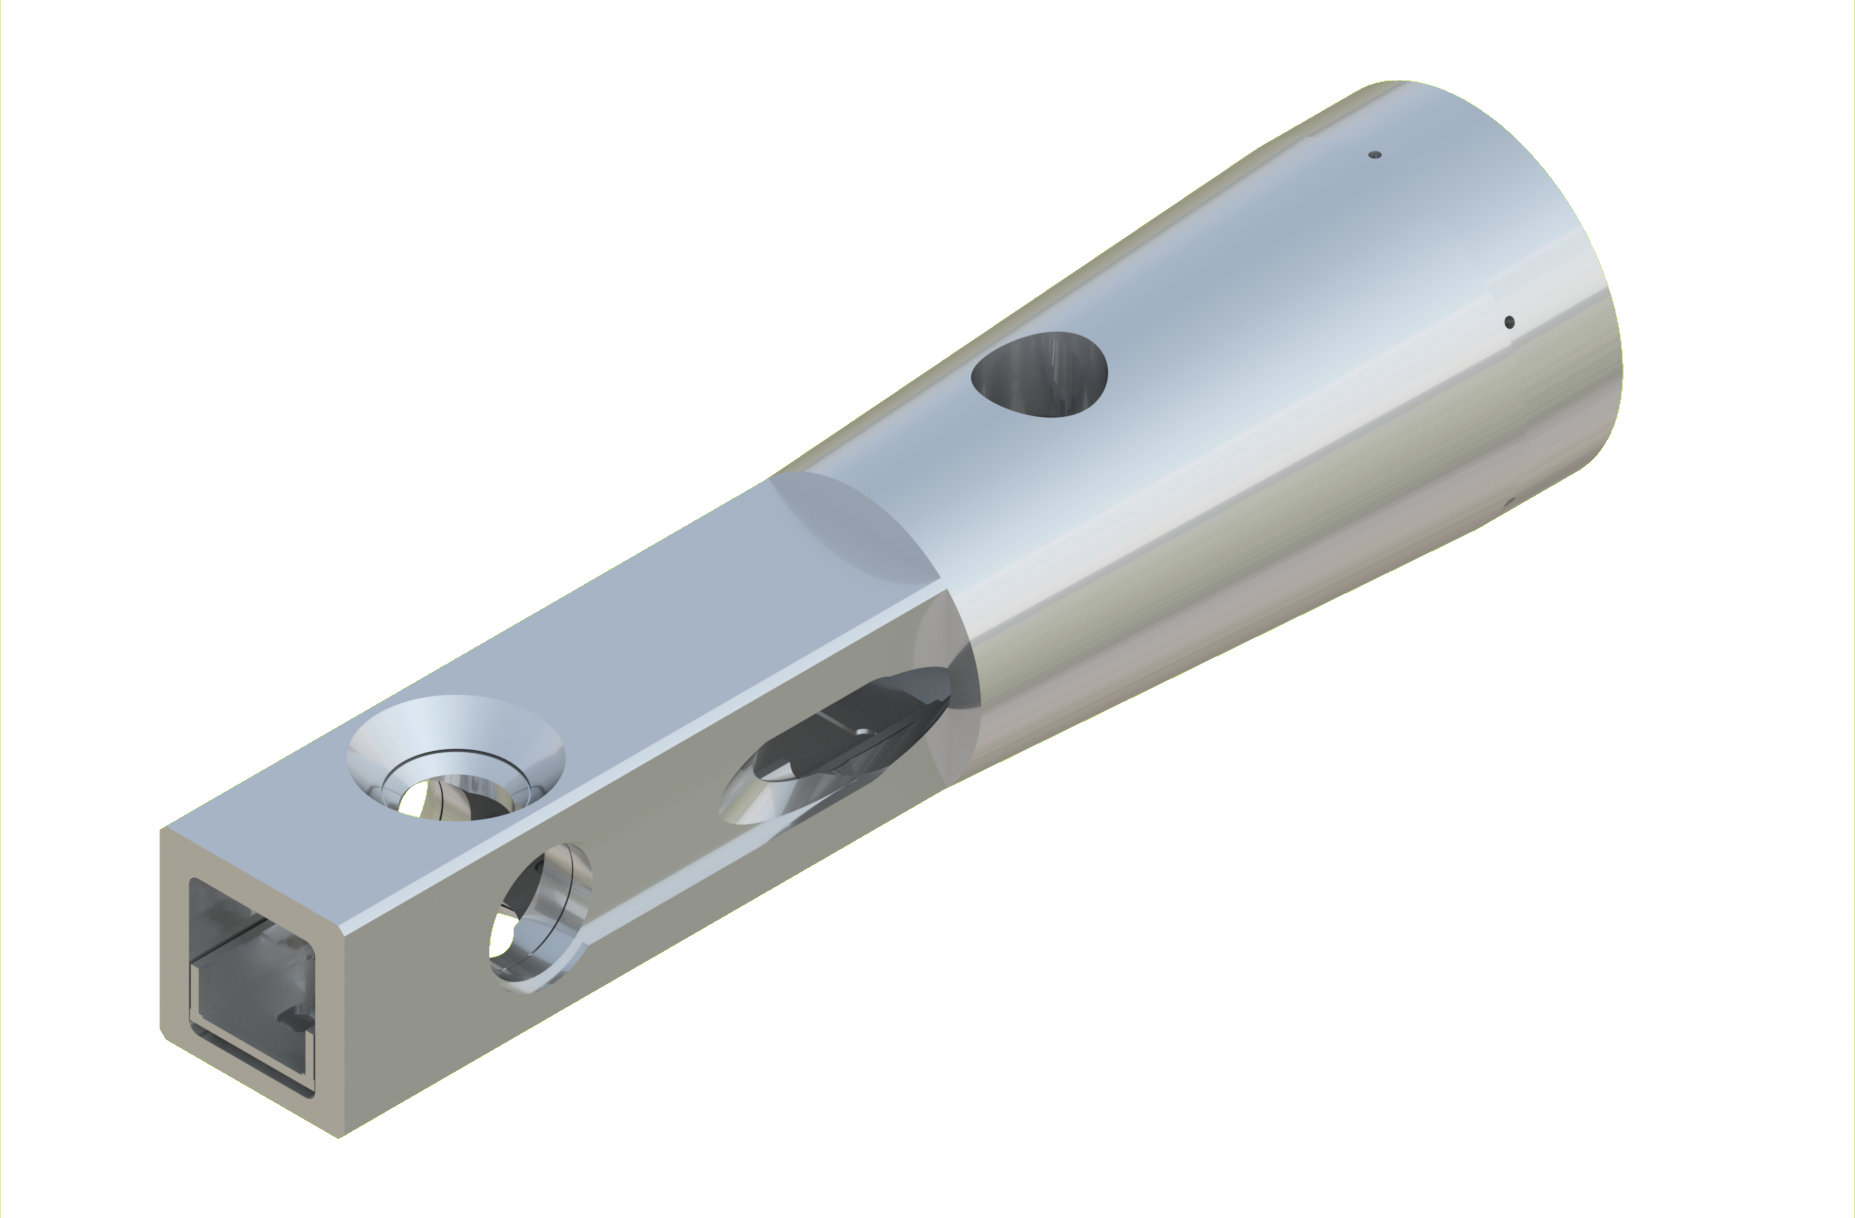
\includegraphics[width=3.5cm]{FINALFINGERtrans.png}};
	
	\addlegendentry{\footnotesize \hspace{0.3em} $G=\SI{0.1}{\percent}$}
	\addlegendentry{\footnotesize \hspace{0.3em} $G=\SI{1}{\percent}$}
	\addlegendentry{\footnotesize \hspace{0.3em} $G=\SI{5}{\percent}$}
	
	\draw[thick, <->] (rel axis cs: 0.54, 0.8) --++ (150:0.5cm);
	\node[align=left] at (rel axis cs: 0.532, 0.88) {\footnotesize $x$};
	
	\nextgroupplot
	[
	ymode=log,
	ymin=1e-0,
	ymax=1e2,
	%ymin=1e-2, ymax=1e0,
	%xlabel={Frequency},
	ylabel={Maximum linear acceleration magnitude (\si{\milli\meter\per\second\squared})},
	xmin=0, xmax=10,
	xticklabels={,,},
	%ymin=-0.1, ymax=1.1,
	%ymin=0, ymax=120,
	%xtick={0,20,40,60,80,100},
	%ytick={0,20,40,60,80,100,120},
	%legend pos=north west,
	ymajorgrids=true,
	xmajorgrids=true,
	grid style=dashed,
	legend cell align={left},
	legend style={
		at={(1, 1)},  % Adjust (x, y) to move it
		anchor=north east,  % Attach the legend to its top-right corner
		draw=none,           % Optional: Remove border around the legend
		fill=none,
		align=left
	}
	]
	
	%\node[align=center] at (axis cs: 1.890, 3500) {\footnotesize A};
	\node[align=center] at (axis cs: 1.979, 6) {\footnotesize\sc b};
	\node[align=center] at (axis cs: 5.893, 20) {\footnotesize\sc c};
	\node[align=center] at (axis cs: 6.337, 61) {\footnotesize\sc d};
	\node[align=center] at (axis cs: 6.466, 42) {\footnotesize\sc e};
	\node[align=center] at (axis cs: 8.530, 13) {\footnotesize\sc f};
	
	\addplot[
	color=markrood,
	name path=ypointone,
	] table [col sep = comma, x expr = \thisrowno{0}/1000, y index = 1]{F_y_01.csv};
	
	\addplot[
	color=rainbow2of8,
	name path=yone,
	] table [col sep = comma, x expr = \thisrowno{0}/1000, y index = 1]{F_y_1.csv};
	
	\addplot[
	color=rainbow3of8,
	name path=yfive,
	] table [col sep = comma, x expr = \thisrowno{0}/1000, y index = 1]{F_y_5.csv};
	
	\addplot+[draw=none,domain=0:10,name path=yzero] {0.01}; 
	
	\addplot[color=markrood, opacity=0.5] fill between[
	of = yone and ypointone,
	]; 
	
	\addplot[color=rainbow2of8, opacity=0.5] fill between[
	of = yfive and yone,
	]; 
	
	\addplot[color=rainbow3of8, opacity=0.5] fill between[
	of = yzero and yfive,
	]; 
	
	\node at (rel axis cs: 0.37, 0.65) [anchor=center] {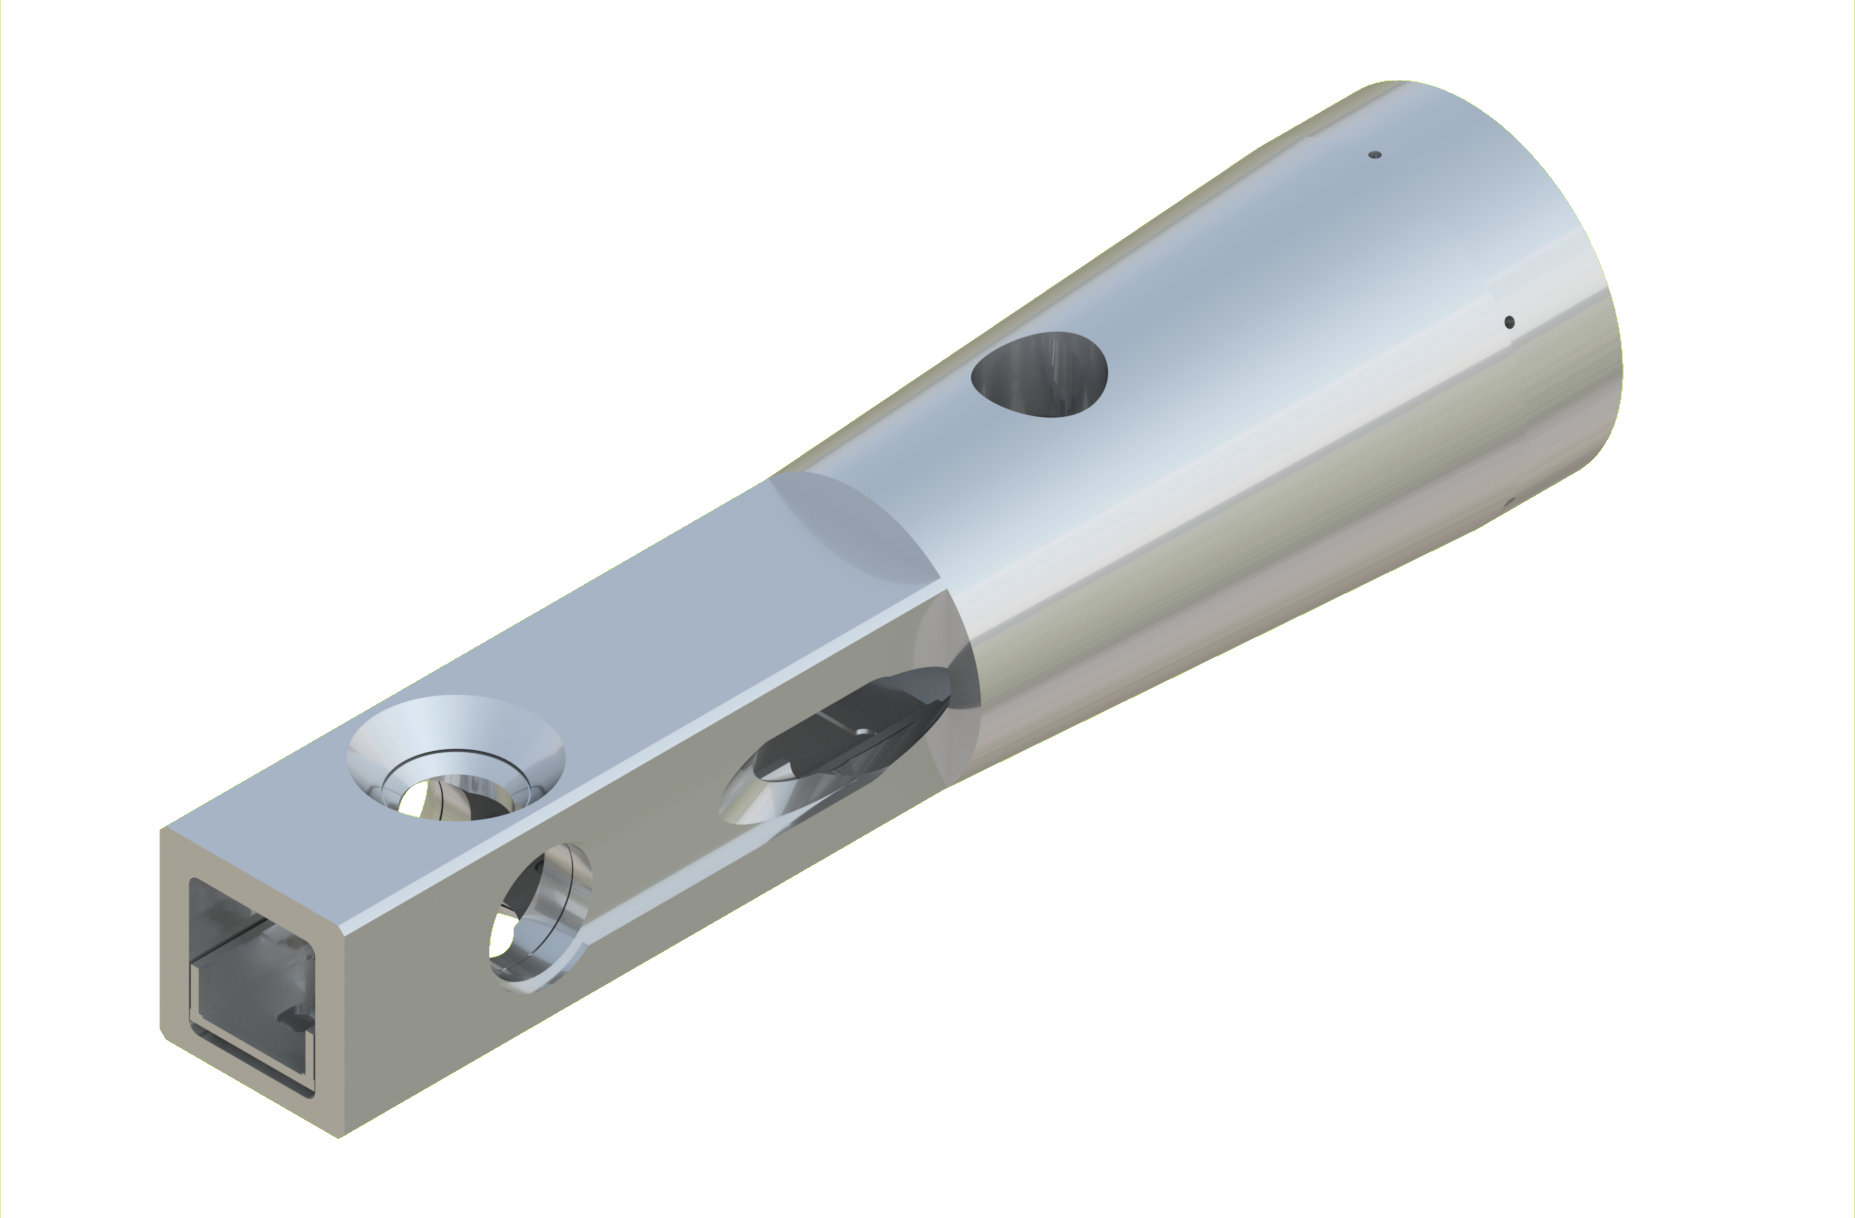
\includegraphics[width=3.5cm]{FINALFINGERtrans.png}};
	
	%\addlegendentry{\small \hspace{0.3em} $G=\SI{0.1}{\percent}$}
	%\addlegendentry{\small \hspace{0.3em} $G=\SI{1}{\percent}$}
	%\addlegendentry{\small \hspace{0.3em} $G=\SI{5}{\percent}$}
	
	\draw[thick, <->] (rel axis cs: 0.505, 0.81) --++ (30:0.5cm);
	\node[align=left] at (rel axis cs: 0.515, 0.895) {\footnotesize $y$};
	
	\nextgroupplot
	[
	ymode=log,
	ymin=1e-0,
	ymax=1e4,
	%ymin=1e-2, ymax=1e0,
	xlabel={Enforced acceleration frequency (\si{\kilo\hertz})},
	%ylabel={Max. linear acceleration},
	xmin=0, xmax=10,
	%ymin=-0.1, ymax=1.1,
	%ymin=0, ymax=120,
	%xtick={0,20,40,60,80,100},
	%ytick={0,20,40,60,80,100,120},
	%legend pos=north west,
	ymajorgrids=true,
	xmajorgrids=true,
	grid style=dashed,
	legend cell align={left},
	legend style={
		at={(1, 1)},  % Adjust (x, y) to move it
		anchor=north east,  % Attach the legend to its top-right corner
		draw=none,           % Optional: Remove border around the legend
		fill=none,
		align=left
	}
	]
	
	\node[align=center] at (axis cs: 1.890, 3500) {\footnotesize\sc a};
	%\node[align=center] at (axis cs: 1.979, 3500) {\footnotesize B};
	\node[align=center] at (axis cs: 5.893, 55) {\footnotesize\sc c};
	\node[align=center] at (axis cs: 6.337, 5000) {\footnotesize\sc d};
	\node[align=center] at (axis cs: 6.466, 2500) {\footnotesize\sc e};
	\node[align=center] at (axis cs: 8.530, 300) {\footnotesize\sc f};
	
	\addplot[
	color=markrood,
	name path=zpointone,
	] table [col sep = comma, x expr = \thisrowno{0}/1000, y index = 1]{F_z_01.csv};
	
	\addplot[
	color=rainbow2of8,
	name path=zone,
	] table [col sep = comma, x expr = \thisrowno{0}/1000, y index = 1]{F_z_1.csv};
	
	\addplot[
	color=rainbow3of8,
	name path=zfive,
	] table [col sep = comma, x expr = \thisrowno{0}/1000, y index = 1]{F_z_5.csv};
	
	\addplot+[draw=none,domain=0:10,name path=zzero] {0.01}; 
	
	\addplot[color=markrood, opacity=0.5] fill between[
	of = zone and zpointone,
	]; 
	
	\addplot[color=rainbow2of8, opacity=0.5] fill between[
	of = zfive and zone,
	]; 
	
	\addplot[color=rainbow3of8, opacity=0.5] fill between[
	of = zzero and zfive,
	]; 
	
	\node at (rel axis cs: 0.37, 0.65) [anchor=center] {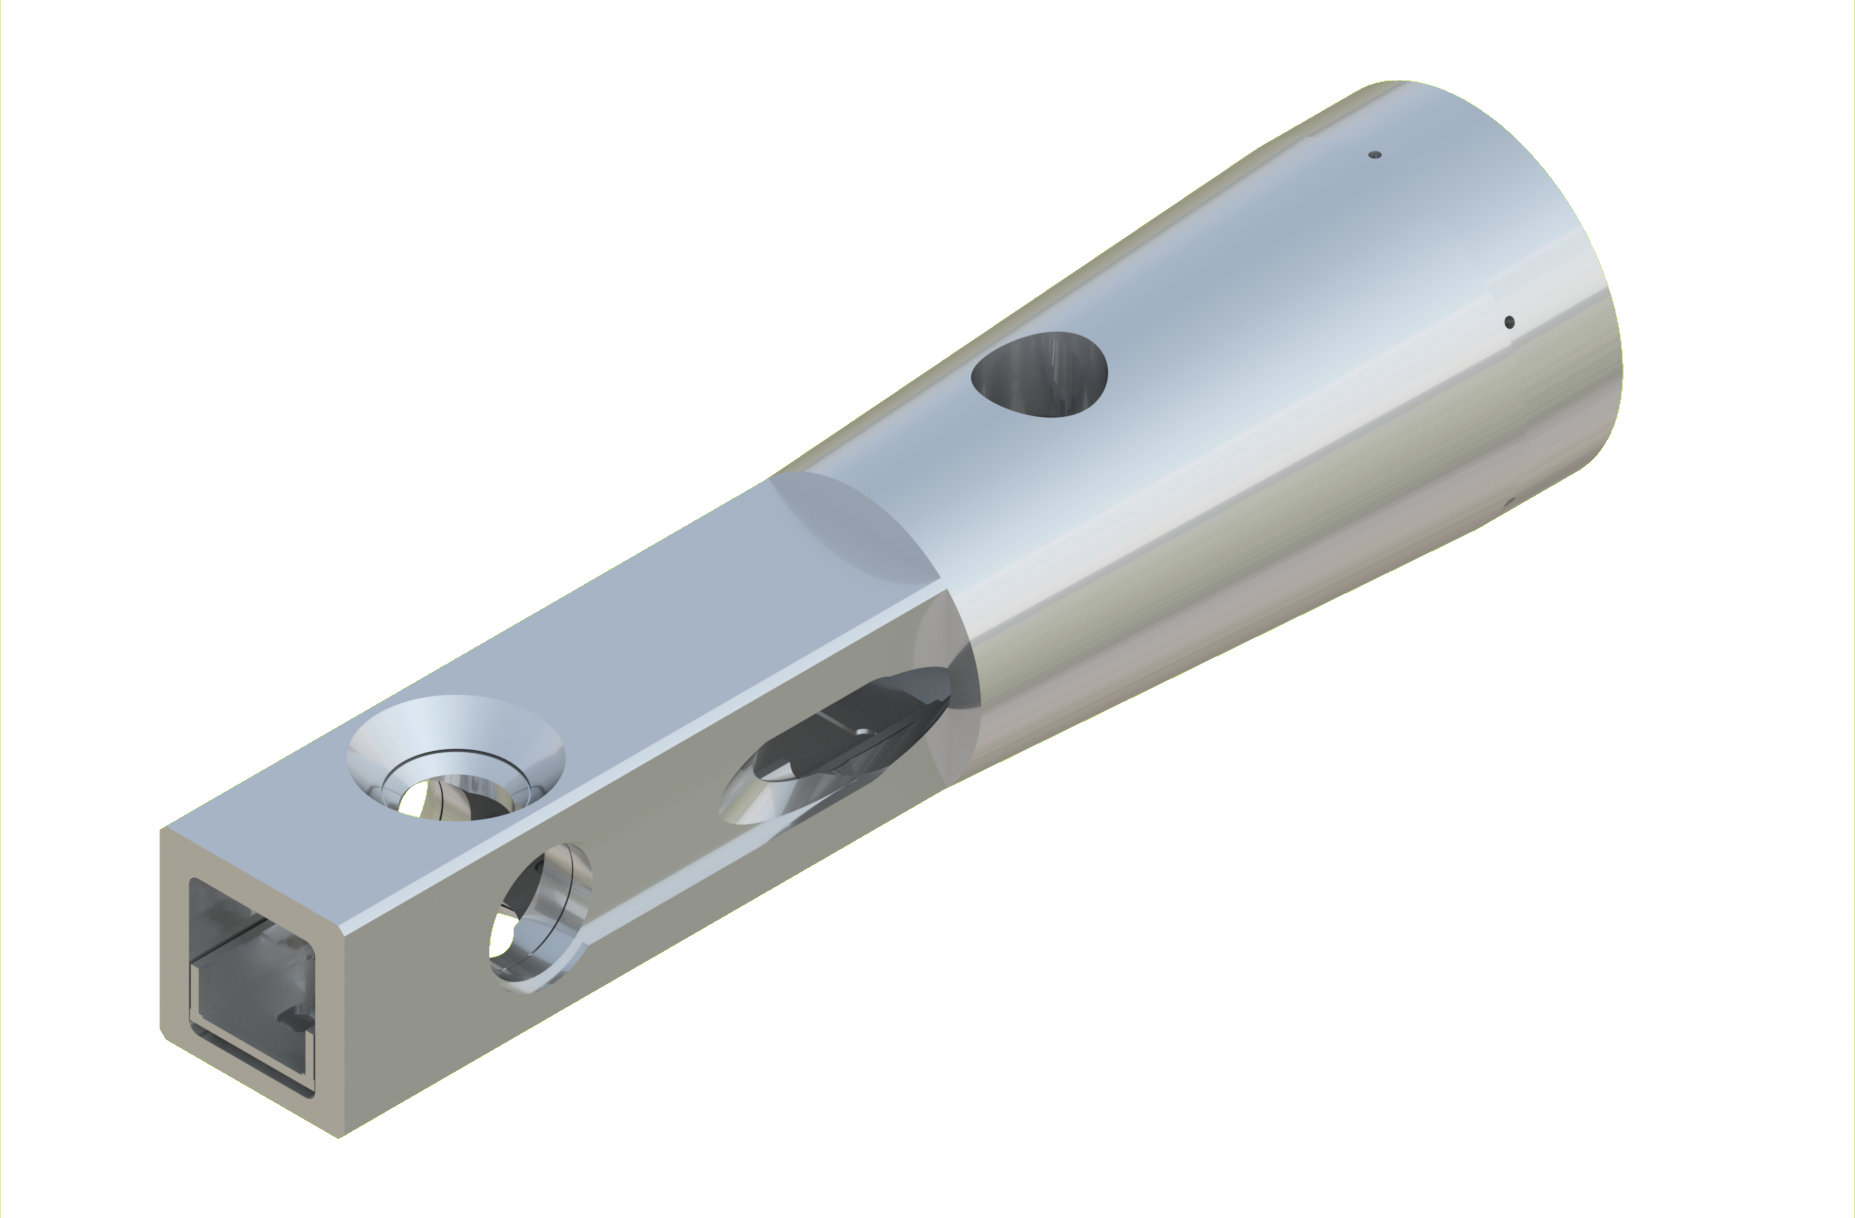
\includegraphics[width=3.5cm]{FINALFINGERtrans.png}};
	
	\draw[thick, <->] (rel axis cs: 0.515, 0.79) --++ (90:0.5cm);
	\node[align=left] at (rel axis cs: 0.535, 0.86) {\footnotesize $z$};
	
	%\addlegendentry{\small \hspace{0.3em} $G=\SI{0.1}{\percent}$}
	%\addlegendentry{\small \hspace{0.3em} $G=\SI{1}{\percent}$}
	%\addlegendentry{\small \hspace{0.3em} $G=\SI{5}{\percent}$}
	
	\end{groupplot}
	
	
	
	\end{tikzpicture}
	\caption[Modal frequency response analysis for glass-substrate cavity mounting structure]{Modal frequency response analysis for glass-substrate cavity mounting structure. The graphs show the maximum linear acceleration magnitude of the structure versus the frequency of enforced acceleration at the base in three different directions: $x$ (top), $y$ (middle) and $z$ (bottom). In each direction, traces are shown for three different values of the structural damping coefficient $G$. The magnitude of the enforced acceleration equals \SI{1}{\milli\meter\per\second\squared}}
	\label{freqresponseFF} 
\end{figure}



\begin{figure}[t]
	\vspace{0em}
	\centering
	\begin{subfigure}[b]{.45\linewidth}
		\begin{tikzpicture}
		\centering
		\node[inner sep=0] (image) at (0,0) {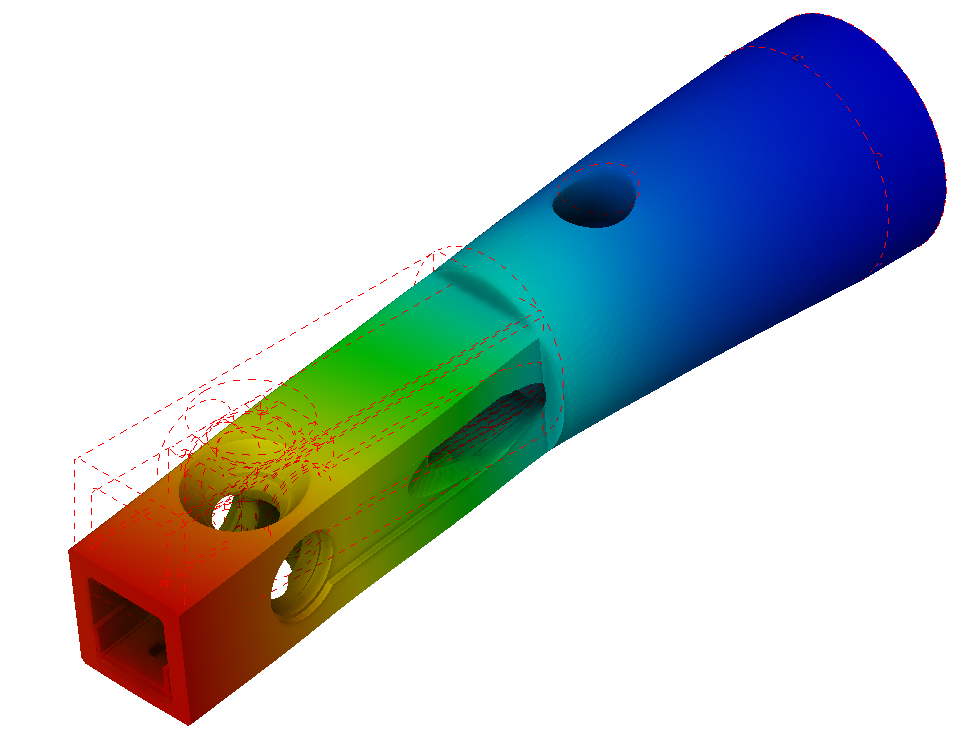
\includegraphics[width=5cm] {F1F.png}};;
		\begin{scope}[x={(image.south east)},y={(image.north west)}]
		\node at (0.2, 0.7) {\footnotesize \SI{1890}{\hertz}};
		\end{scope}
		\end{tikzpicture}
		\centering
		\caption{}
		\label{a}
	\end{subfigure}
	\begin{subfigure}[b]{.45\linewidth}
		\begin{tikzpicture}
		\centering
		\node[inner sep=0] (image) at (0,0) {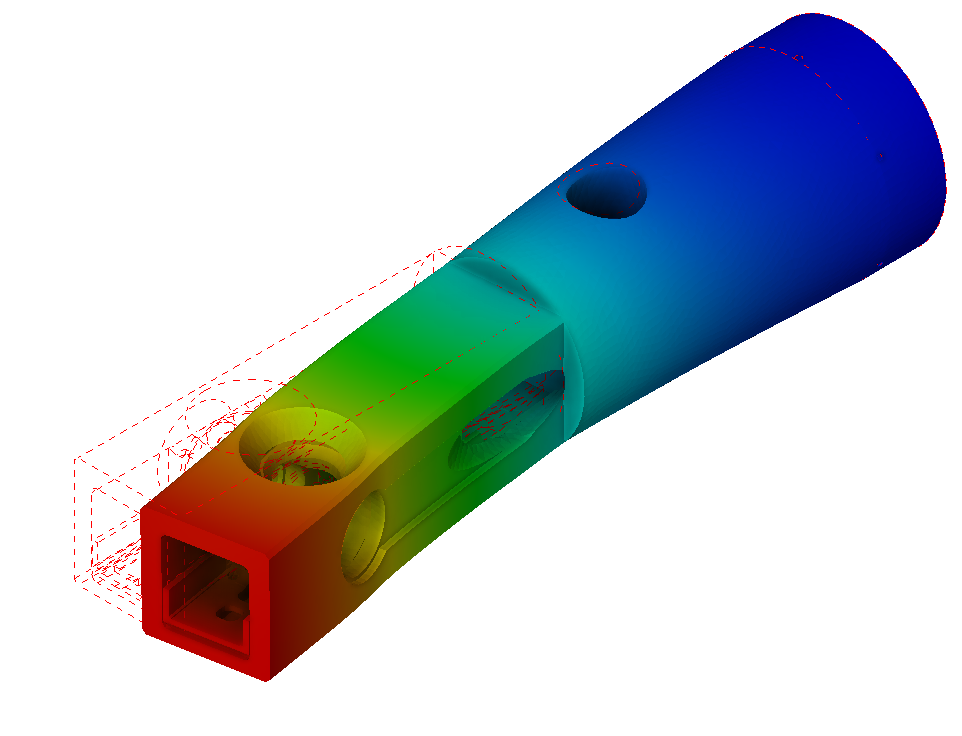
\includegraphics[width=5cm] {F2F.png}};;
		\begin{scope}[x={(image.south east)},y={(image.north west)}]
		\node at (0.2, 0.7) {\footnotesize \SI{1979}{\hertz}};
		\end{scope}
		\end{tikzpicture}
		\centering
		\caption{}
		\label{b}
	\end{subfigure}
	\\
	\begin{subfigure}[b]{.45\linewidth}
		\begin{tikzpicture}
		\centering
		\node[inner sep=0] (image) at (0,0) {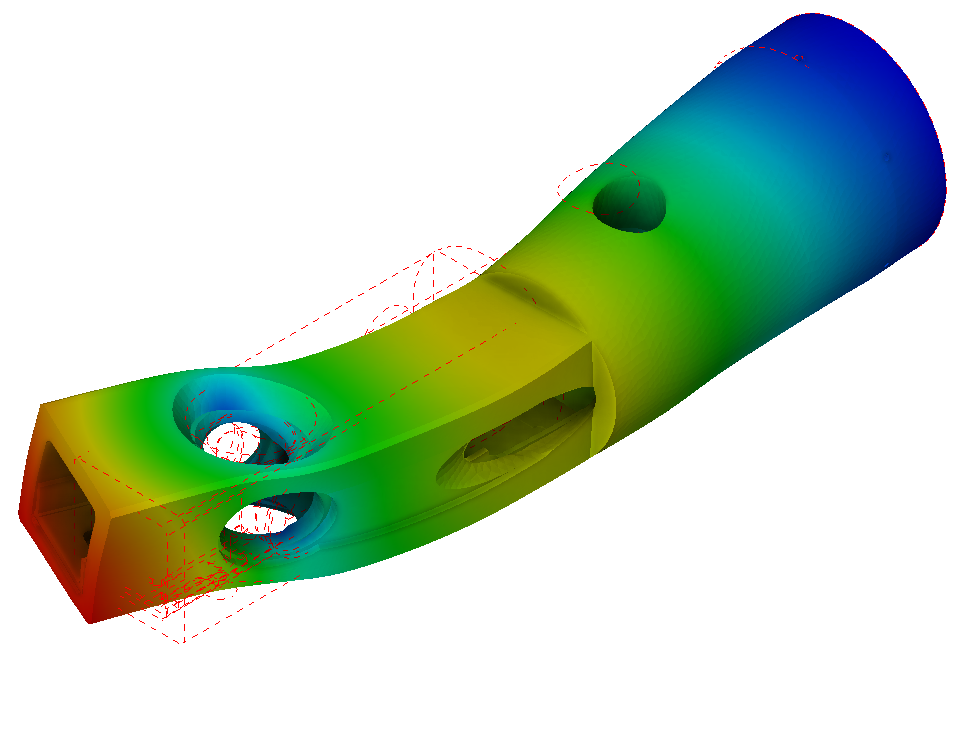
\includegraphics[width=5cm] {F3F.png}};;
		\begin{scope}[x={(image.south east)},y={(image.north west)}]
		\node at (0.2, 0.7) {\footnotesize \SI{5893}{\hertz}};
		\end{scope}
		\end{tikzpicture}
		\centering
		\caption{}
		\label{c}
	\end{subfigure}
	\begin{subfigure}[b]{.45\linewidth}
		\begin{tikzpicture}
		\centering
		\node[inner sep=0] (image) at (0,0) {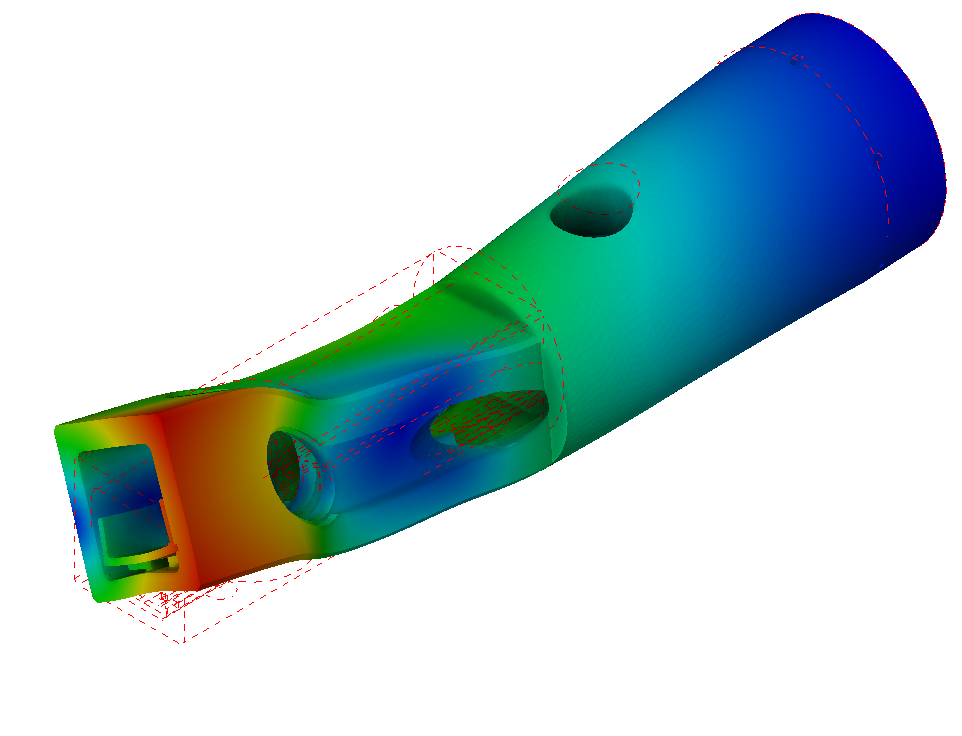
\includegraphics[width=5cm] {F4F.png}};;
		\begin{scope}[x={(image.south east)},y={(image.north west)}]
		\node at (0.2, 0.7) {\footnotesize \SI{6337}{\hertz}};
		\end{scope}
		\end{tikzpicture}
		\centering
		\caption{}
		\label{c}
	\end{subfigure}
	\\
	\begin{subfigure}[b]{.45\linewidth}
		\begin{tikzpicture}
		\centering
		\node[inner sep=0] (image) at (0,0) {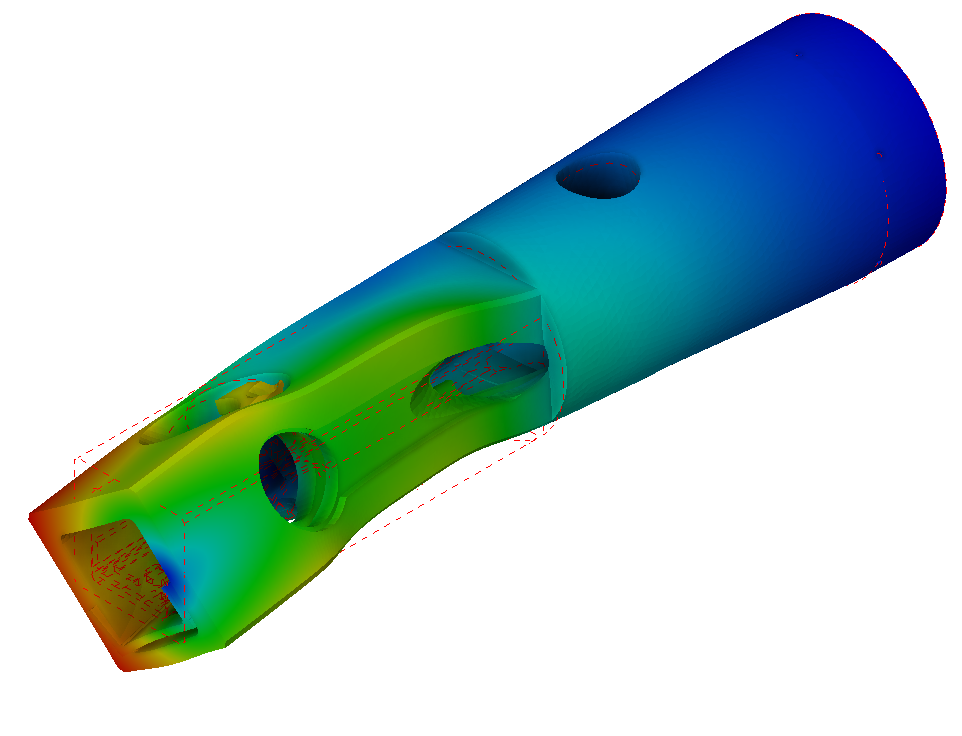
\includegraphics[width=5cm] {F5F.png}};;
		\begin{scope}[x={(image.south east)},y={(image.north west)}]
		\node at (0.2, 0.7) {\footnotesize \SI{6466}{\hertz}};
		\end{scope}
		\end{tikzpicture}
		\centering
		\caption{}
		\label{a}
	\end{subfigure}
	\begin{subfigure}[b]{.45\linewidth}
		\begin{tikzpicture}
		\centering
		\node[inner sep=0] (image) at (0,0) {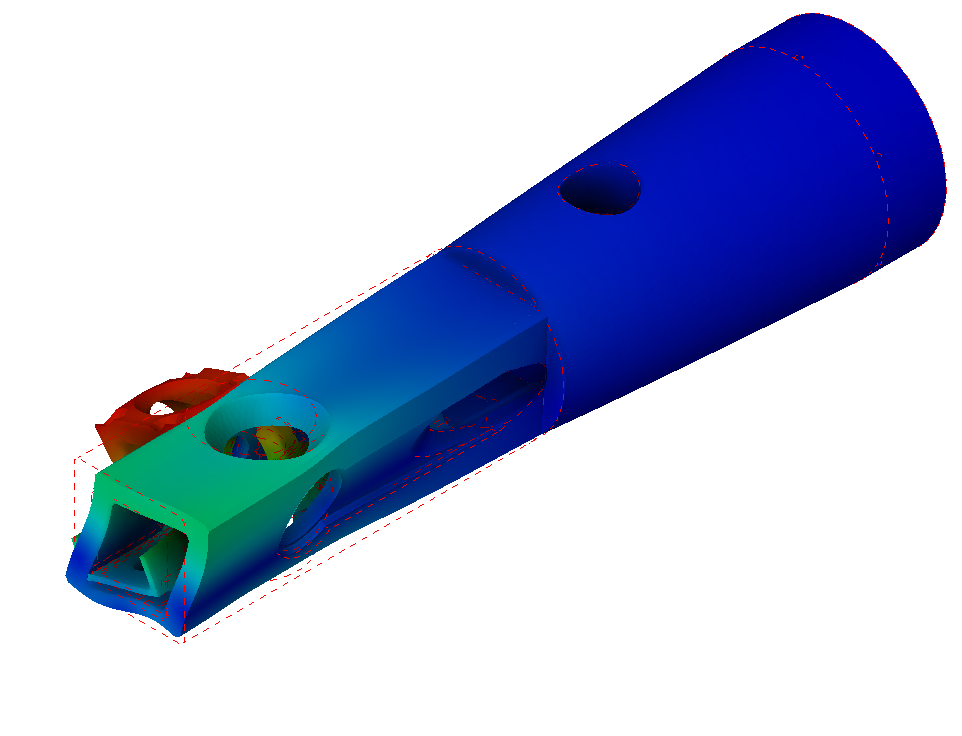
\includegraphics[width=5cm] {F6F.png}};;
		\begin{scope}[x={(image.south east)},y={(image.north west)}]
		\node at (0.2, 0.7) {\footnotesize \SI{8530}{\hertz}};
		\draw[thick, ->] (1, 0.15) --++ (90:0.5cm) node[above, anchor=south] {\footnotesize $z$};
\draw[thick, ->] (1, 0.15) --++ (150:0.5cm) node[above, anchor=base] {\footnotesize  $x$\,\, \phantom{x}};
\draw[thick, ->] (1, 0.15) --++ (210:0.5cm) node[above, anchor=mid] {\footnotesize $y$\,\, \phantom{x}};
		\end{scope}
		\end{tikzpicture}
		\centering
		\caption{}
		\label{b}
	\end{subfigure}
	\caption[Normal modes below \SI{10}{\kilo\hertz} for glass-substrate cavity mounting structure]{Normal modes and corresponding frequencies below \SI{10}{\kilo\hertz} for the glass-substrate cavity mounting structure. The colour scale corresponds to the displacement from the unperturbed position of the structure (dashed contours). Mode labels correspond to those in \autoref{freqresponseFF}.}
	\label{FFmodes}
\end{figure}

\begin{table}[h]
	\centering
	\begin{tabular}{ccccccc}
		\toprule
		{Mode number} & { ${T}_x$} & {${T}_y$} & {${T}_z$} & {${R}_x$} & {${R}_y$} & {${R}_z$} \\
		\midrule
		1 (\textsc{a}) & 0.0007 & 0.0000 & 35.8125 & 1.5245 & 0.0004 & 0.0000 \\
		2 (\textsc{b}) & 35.7347 & 0.0001 & 0.0007 & 0.0000 & 0.0006 & 1.5554 \\
		3 (\textsc{c}) & 26.7161 & 0.0023 & 0.0092 & 0.0073 & 0.2986 & 25.4059 \\
		4 (\textsc{d}) & 0.1826 & 0.0070 & 19.8976 & 19.7244 & 8.5420 & 1.1956 \\
		5 (\textsc{e}) & 0.2574 & 0.0023 & 7.2673 & 7.7576 & 15.4124 & 0.2826 \\
		6 (\textsc{f}) & 0.0940 & 0.0001 & 0.0290 & 0.0322 & 1.1623 & 0.1025 \\
		7 & 0.0120 & 1.0386 & 10.8091 & 15.2692 & 0.7660 & 0.0199 \\
		8 & 0.1064 & 45.3301 & 0.2023 & 0.2995 & 0.0543 & 0.1714 \\
		9 & 8.2676 & 0.5778 & 0.0307 & 0.0477 & 10.6172 & 13.3469 \\
		10 & 3.8187 & 0.2649 & 0.0035 & 0.0056 & 26.4222 & 6.3842 \\
		\midrule
		{Total} & 75.1903 & 47.2232 & 74.0620 & 44.6679 & 63.2762 & 47.4645 \\
		\bottomrule
	\end{tabular}
\caption[Percentages of modal effective mass for cavity (glass-substrate) mounting structure]{Modal effective mass participation for the first 10 modes of the cavity (glass-substrate) mounting structure. The numbers shown represent percentages for the translational (${T}_x$, ${T}_y$, ${T}_z$) and rotational (${R}_x$, ${R}_y$, ${R}_z$) degrees of freedom. Labels are references to the modes as indicated in \autoref{freqresponseFF} and \autoref{FFmodes}.}
	\label{tab:modepercentFinalfinger}   
\end{table}







\section{PYRAMID MOT}

For the operation of holographic optical tweezers inside a cavity (see \autoref{exp5}), it is not possible to load microtraps from a MOT positioned between the cavity mirrors due to limited optical access for the MOT beams. The idea is to position the MOT cloud in the neighbourhood of the cavity, from which atoms are then transported towards the focal plane of the trapping light inside the cavity. There are various methods of doing this, which include funnelling atoms ejected with an atomic fountain using a combination of blue detuned cavity modes \cite{Puppe2007}, guiding atoms from a static MOT with a single, red detuned beam \cite{Numann2005} or using an optical lattice that can act as an optical conveyor belt \cite{Gallego2018,Schrader2001}. For this experiment, we propose using an atomic fountain to load a large grid of holographic microtraps in the cavity. This will increase the capture probability from the thermally expanding cloud of atoms.

\begin{figure}[!t]
	\center
	\includegraphics[width=0.75\linewidth]{{"motdiffraction"}.pdf}
	\caption[asdf]{}
	\label{fig:BreitRabiDiagram} 
\end{figure}

\begin{figure}[t]
	\hspace{-0cm}
	\begin{tikzpicture}[remember picture]
	\node[anchor=south west,inner sep=0] (image1) at (0,0) {\includegraphics[width=1\textwidth]{{"pyramidinfinger"}.pdf}};
	
	% left four
	\begin{scope}[x={(image1.south east)},y={(image1.north west)}]
	% draw a grid
	%\draw[help lines,xstep=.1,ystep=.1,overlay] (0,0) grid (1,1);
	% draw ticks
	%\foreach \x in {0,1,...,9} { \node [anchor=north,overlay] at (\x/10,0) {0.\x}; }
	%\foreach \y in {0,1,...,9} { \node [anchor=east,overlay] at (0,\y/10) {0.\y}; }
	
	% labels
	%\node[markgrijs, align=center, rotate=0] at (0.0,0.9) {\footnotesize\sc (a)};
	%\node[markgrijs, align=center, rotate=0] at (0.35,0.9) {\footnotesize\sc (b)};
	%\node[markgrijs, align=center, rotate=0] at (0.7,0.9) {\footnotesize\sc (c)};
	
	\node[markgrijs, align=center, rotate=0] at (0.15,0.) {\footnotesize\sc (a)};
	\node[markgrijs, align=center, rotate=0] at (0.5,0.) {\footnotesize\sc (b)};
	\node[markgrijs, align=center, rotate=0] at (0.85,0.) {\footnotesize\sc (c)};
	
	\end{scope}
	
	\end{tikzpicture}
	\caption[Mirror design of a Fabry-Pérot resonator.]{Mirror design of a Fabry-Pérot resonator. Dielectric mirror coatings are applied to the superpolished (\textsc{a}) or laser-ablated (\textsc{b}) end facets of glass substrates with conical (\textsc{a}) and pyramidal (\textsc{b}) geometries, respectively. The indicated mirror specifications (as reported in \cite{doherty2021a}) are the radius (or radii) of curvature $R_\mathrm{c}$, the intensity transmission coefficient $T$ and total incoherent loss $\mathcal{L}$. A white light interferogram (\textsc{c}) reveals the depth profile of the laser-ablated end facet: a Gaussian dimple with an effective mirror diameter of \SI{100}{\micro\meter} \cite{doherty2021a}. (\textsc{d}) Side view of the resonator with dimensions in millimetres. A magnified view of the end facets indicates the total cavity length and angular aperture ($\theta=\SI{40}{\degree}$).}
	\label{finger} 
\end{figure}


\end{document}
